\chapter{CombinedXbbScore Tagger implementation}

\section{Performance}

\par The Boosted Xbb Tagger is based on a neural network (roughly 10 layers) which uses b-tagging and jet substructure information. 
The classification has three outputs which represents how likely the jet is Higgs, Top and QCD jet.  

\par With different fraction of the the three classes, CombinedXbbScore Tagger is defined as
\begin{equation}
D=ln(\frac{p_H}{(1-f)\times p_{QCD}+f\times p_{top}}),
\end{equation}
where f is the mixing fraction of top jet in the background, and XbbScore Top/Higgs/QCD are the three output of the Xbb Tagger.

\par The performance can be expressed in terms of its receiver operator characteristic (ROC) plot, which shows the change of background rejection as a function of the Higgs boson tagging efficiency. 
Fig.\ref{fig:roctop} compares CombinedXbbScore aggers with different mixing fraction.

\begin{figure}[h]
    \centering
    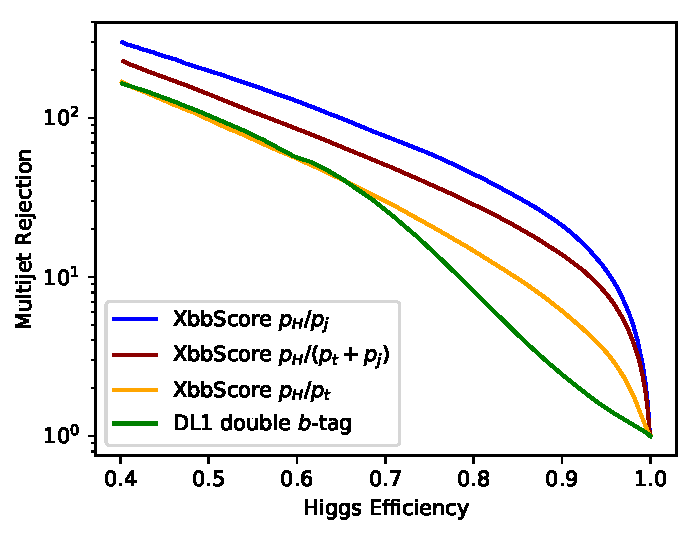
\includegraphics[width=0.4\textwidth]{appendices/figures/roc_multijet.pdf}
    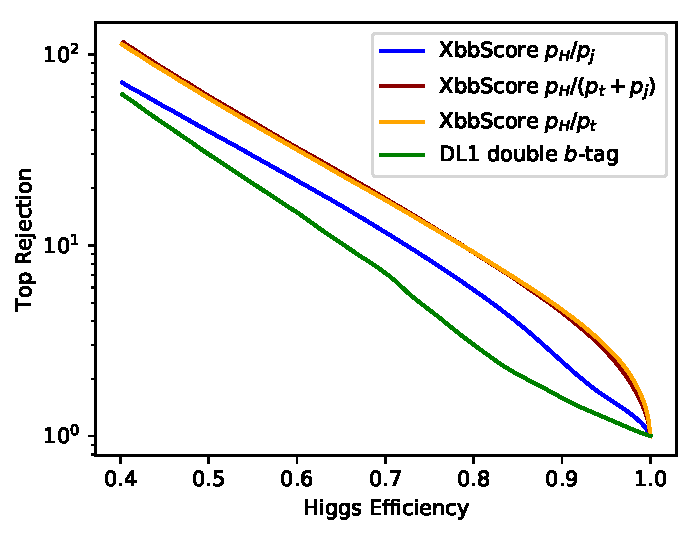
\includegraphics[width=0.4\textwidth]{appendices/figures/roc_top.pdf}
    \caption{ ROC plot: Comparison between different working points of CombinedXbbScore}
    \label{fig:roctop}
\end{figure}

\par The preliminary working points of the CombinedXbbScore are listed in Table.\ref{tab:combxbb}.

\begin{table}
    \footnotesize{
        \begin{center}
            \begin{tabular}{ c |c |c |c}
                \hline
                \hline
                Higgs efficiency [\%] & mixing fraction (f)	& cut value \\
                50 & 0 & 5.1 \\
                60 & 0 & 4.8 \\
                70 & 0 & 3.9 \\
                50 & 0.2 & 4.5 \\
                60 & 0.2 & 3.9 \\
                70 & 0.2 & 3.0 \\
                50 & 1 & 3.6 \\
                60 & 1 & 3.0 \\
                70 & 1 & 2.1 \\
                \hline
                \hline
            \end{tabular}
        \end{center}
        }
    \caption{Preliminary working points of CombinedXbbScore}
    \label{tab:combxbb}
\end{table}

\section{Signal selection in Merged region using CombinedXbbScore}

\par For the merged region, instead of requiring two b-tagged VR trackjets with 77\% working point as described in Section.\ref{sec:ana-sig:physobj}. 
The background large-R jets (R = 1.0) are suppressed by applying a cut on CombinedXbbScore. 
To have a fair comparison within these two methods, 77\% working point is chosen for the VR trackjets b-tagging and 60\% working points are chosen for the CombinedXbbScore tagger with different mixing fractions for all plots showed in this chapter.					

\par The large-R jet mass distribution of the Z’+2HDM signal with $m_Z’ = 2800~GeV$ and $m_A = 300~GeV$ is scaled by a factor of 1000 and compared to backgrounds in both Fig.\ref{fig:mj_before} and Fig.\ref{fig:mj_after}. 	

\par The left plot in Fig.\ref{fig:mj_before} shows the large-R jet mass distribution in the merged region while the right plot shows the large-R jet mass distribution after requiring two b-tagged VR trackjets. 
Fig.\ref{fig:mj_before} shows the large-R jet mass distribution after applying cutting on CombinedXbbScore with mixing fraction $f=1$ (left) and $f=0$ (right). 	

\begin{figure}[h]
    \centering
    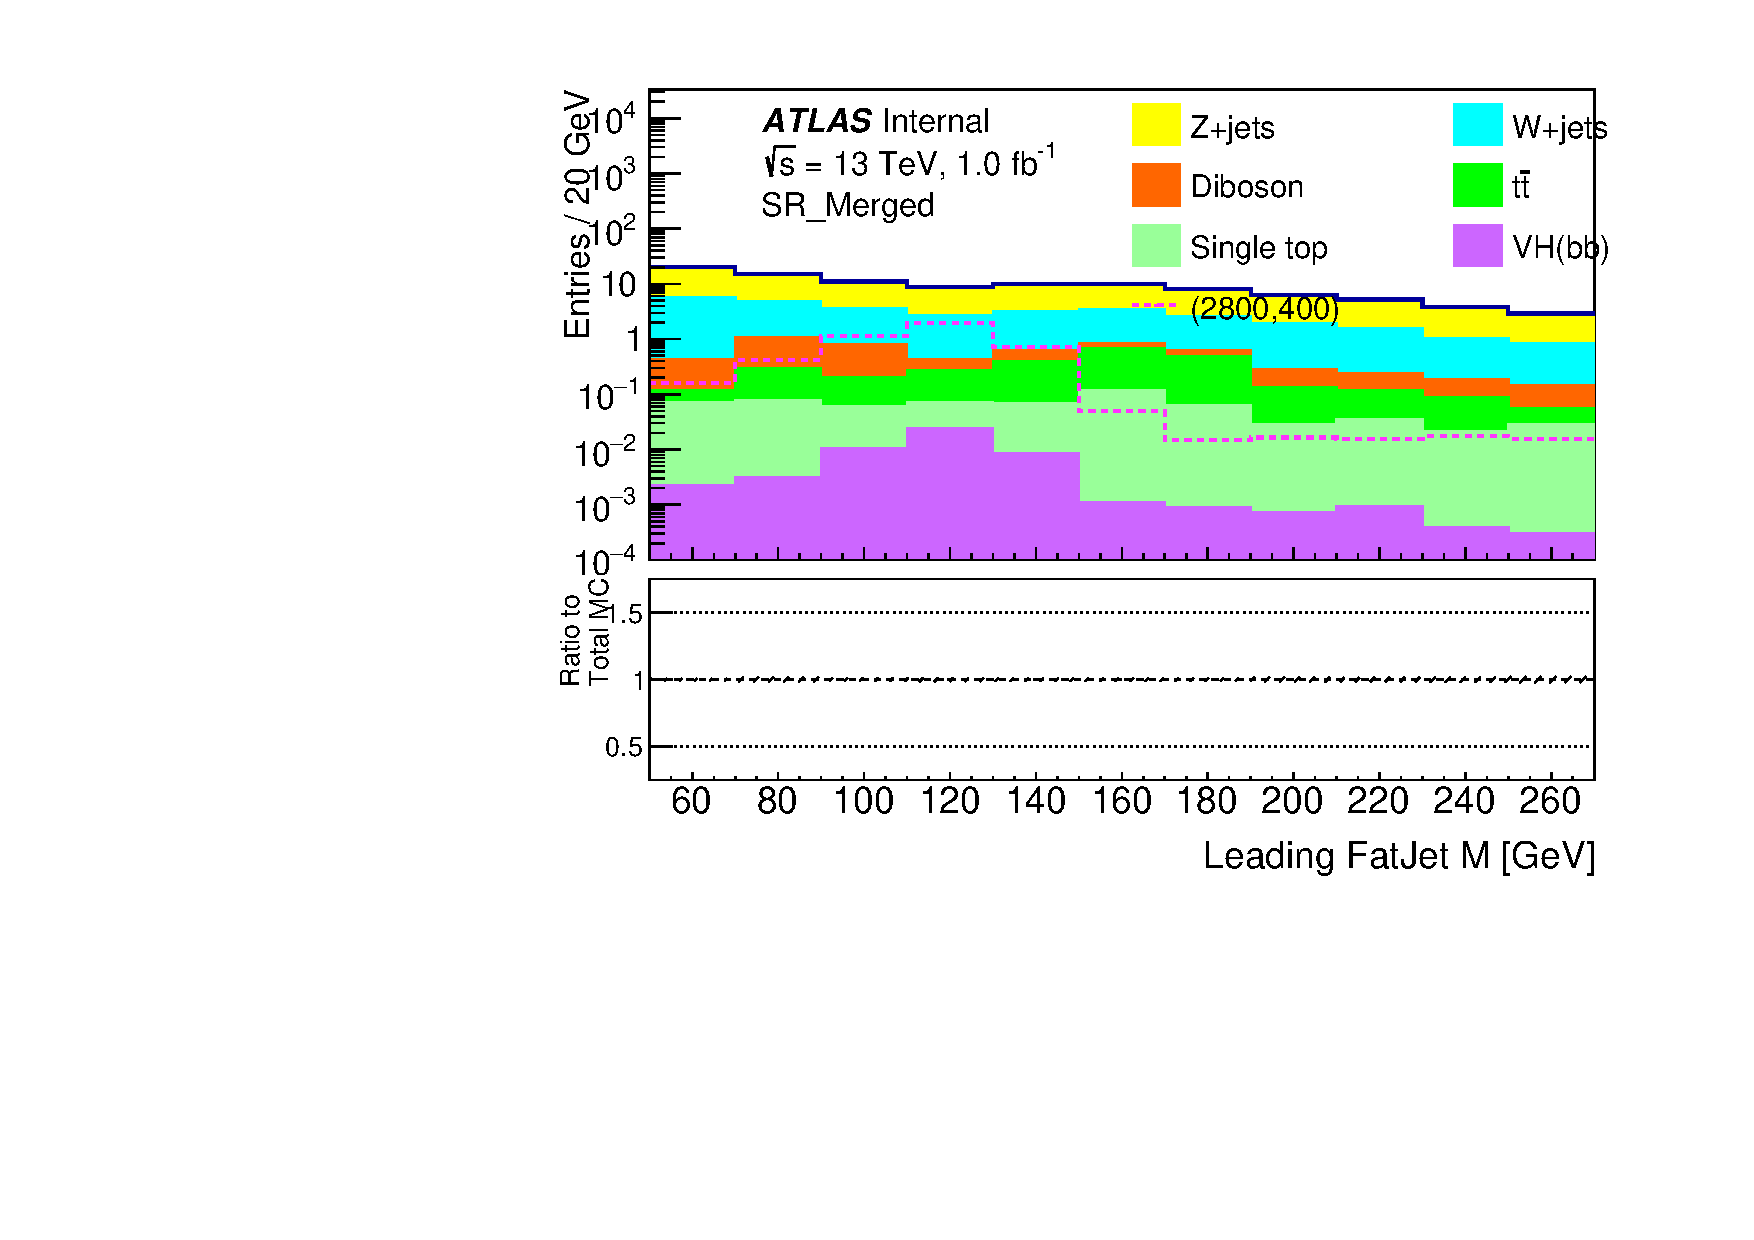
\includegraphics[width=0.4\textwidth]{appendices/figures/MC_MonoH_Nominal_SR_Merged_fatjets_m1_20GeV_LogY.pdf}
    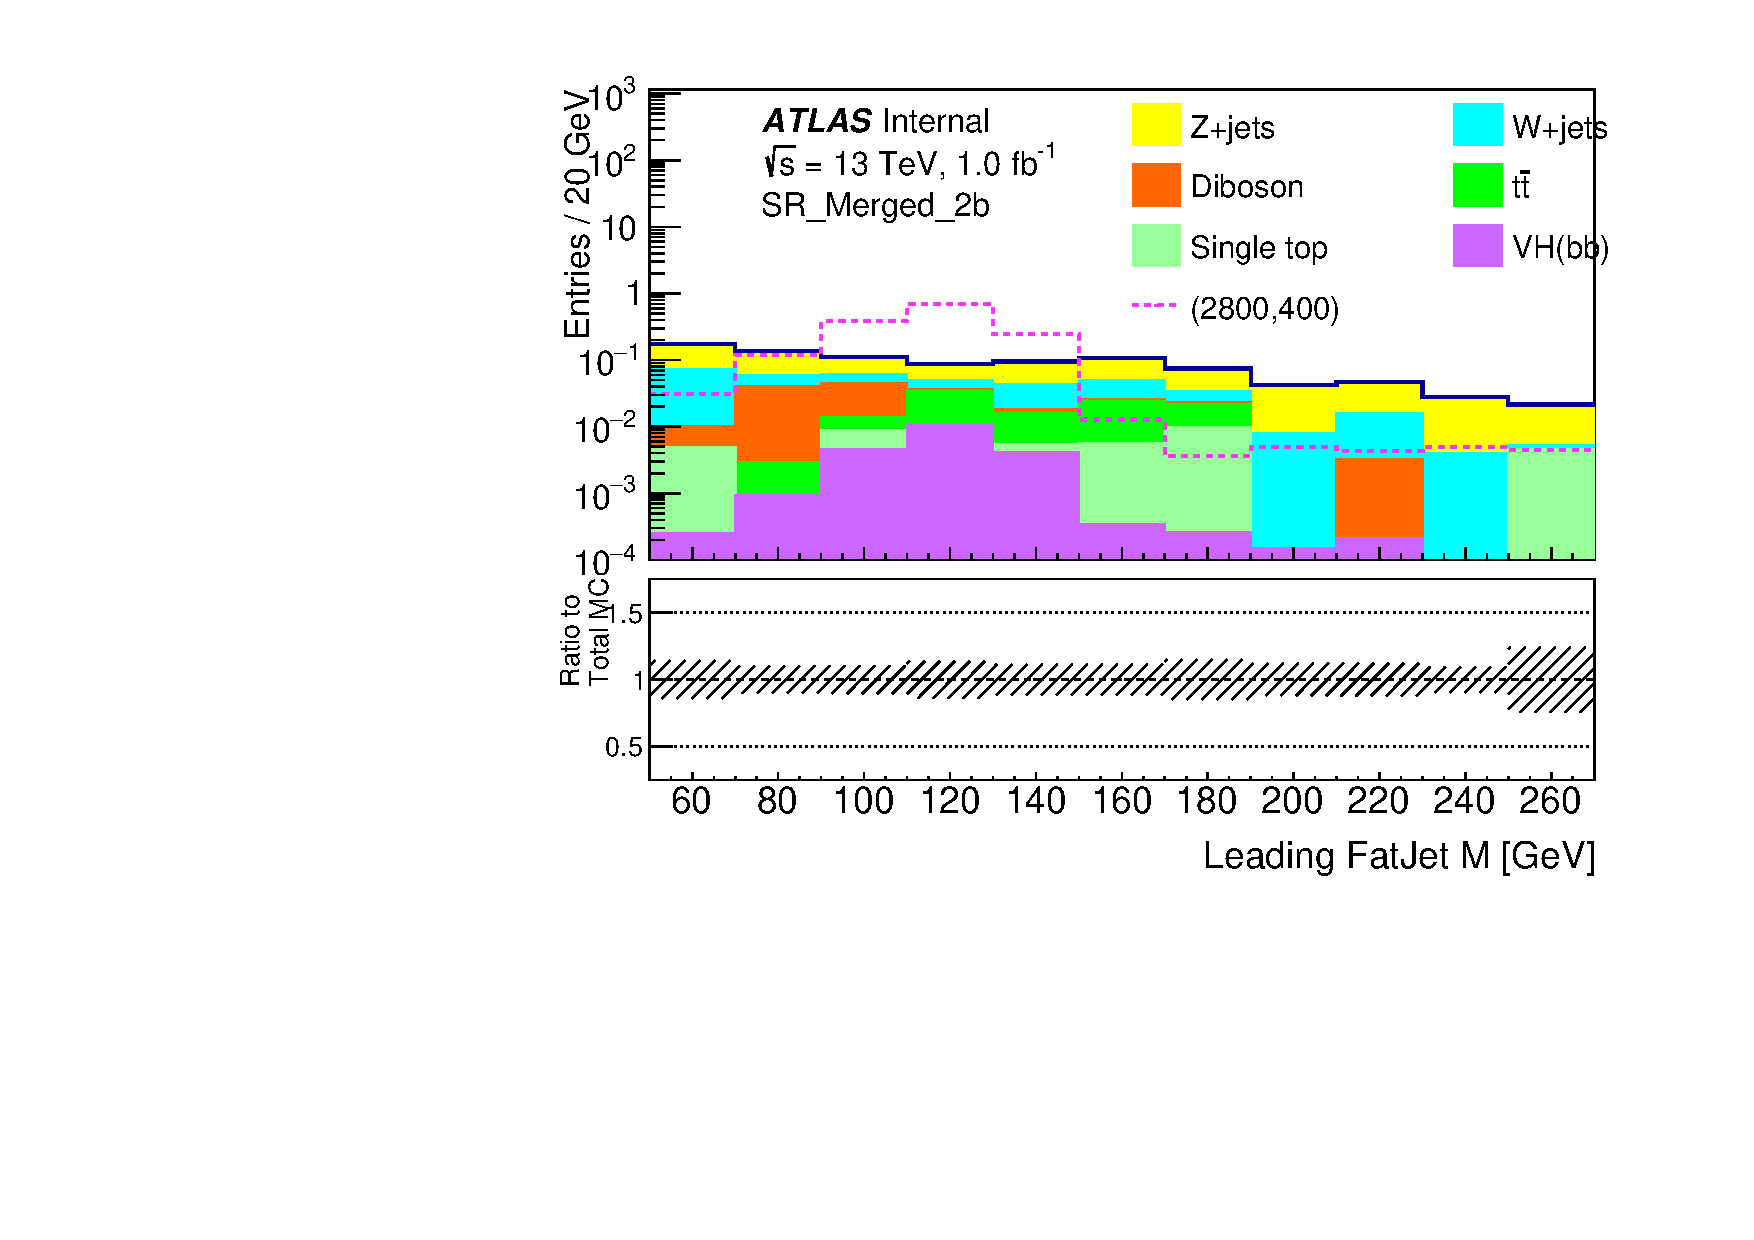
\includegraphics[width=0.4\textwidth]{appendices/figures/MC_MonoH_Nominal_SR_Merged_2b_fatjets_m1_20GeV_LogY_vr.pdf}
    \caption{Leading Fatjet mass in Merged region (left) and 2b Merged region defined by 2-b tagged VR (right)}
    \label{fig:mj_before}
\end{figure}

\begin{figure}[h]
    \centering
    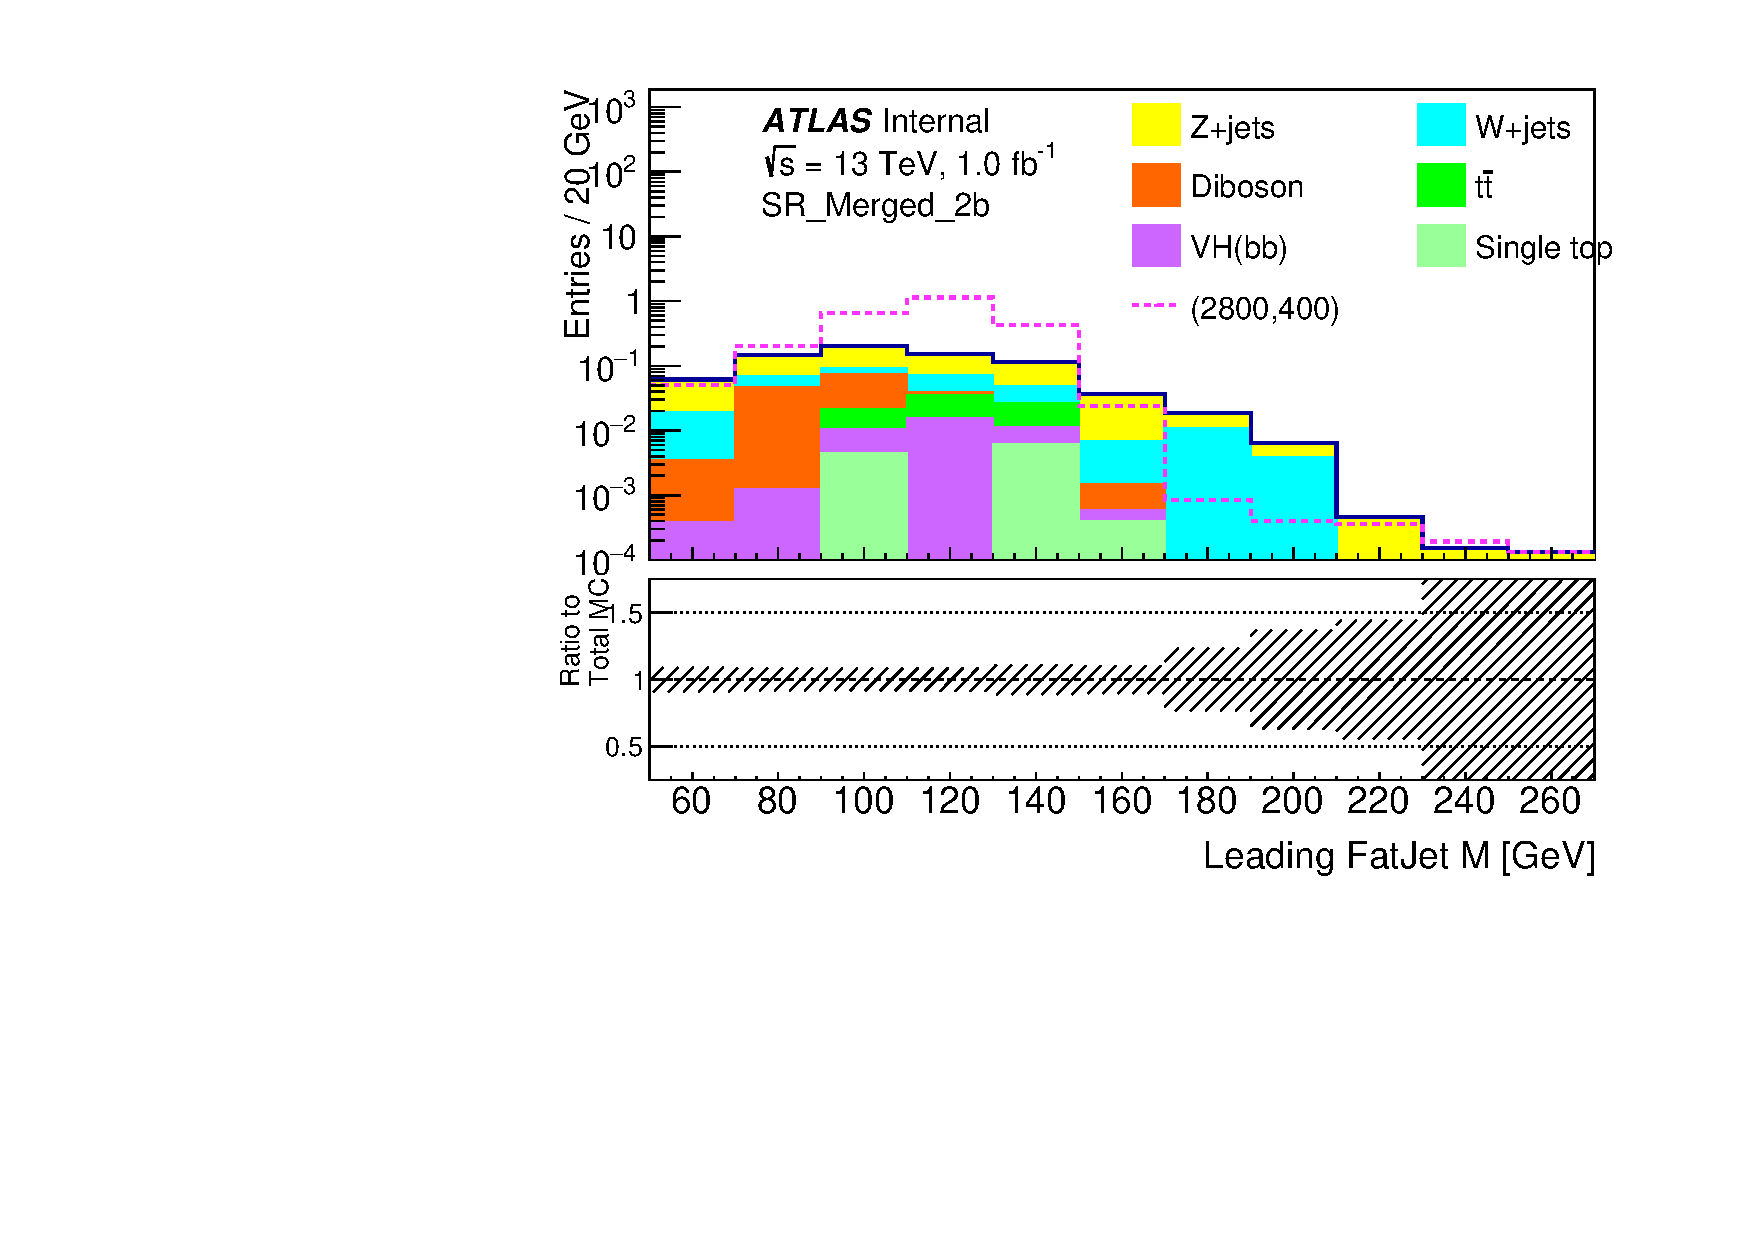
\includegraphics[width=0.4\textwidth]{appendices/figures/MC_MonoH_Nominal_SR_Merged_2b_fatjets_m1_20GeV_LogY_xbb.pdf}
    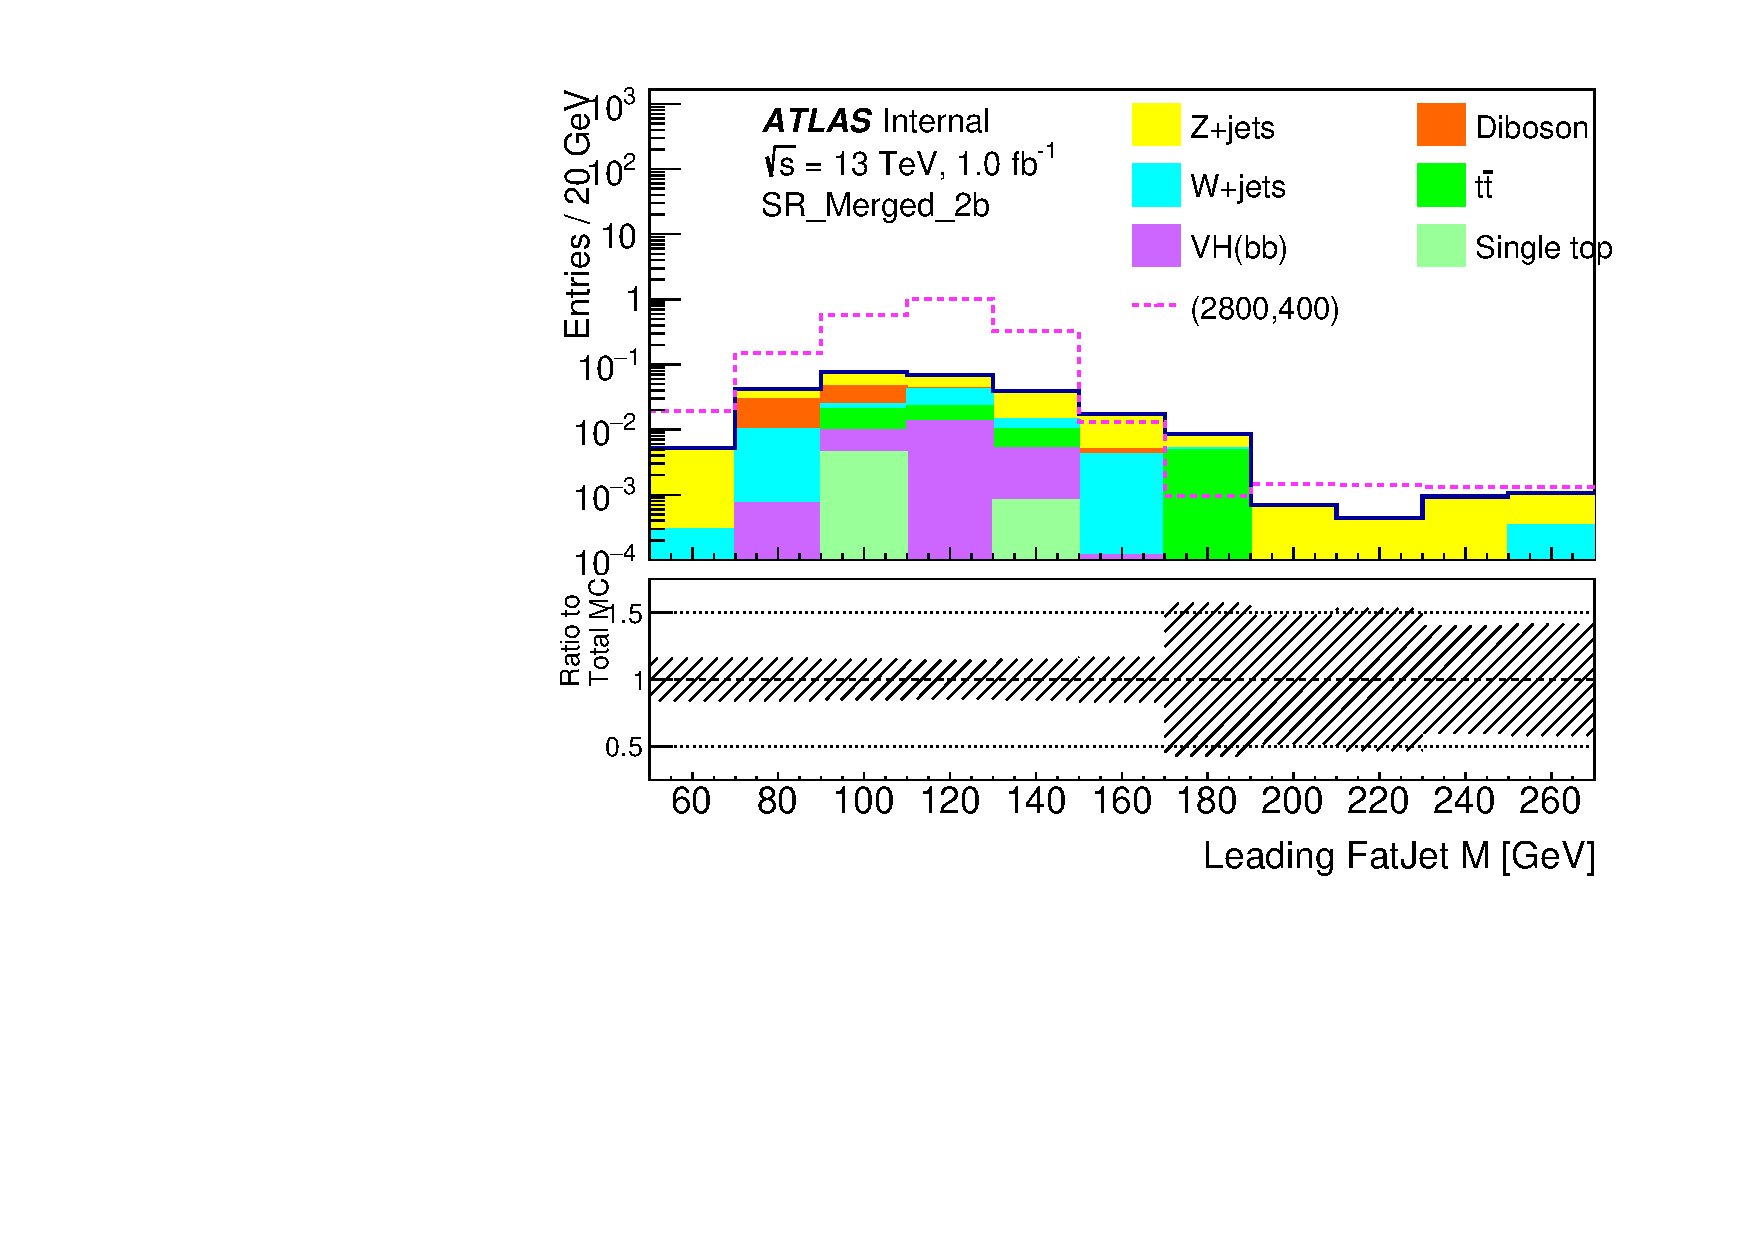
\includegraphics[width=0.4\textwidth]{appendices/figures/MC_MonoH_Nominal_SR_Merged_2b_fatjets_m1_20GeV_LogY_xbb_f0.pdf}
    \caption{Leading Fatjet mass in 2b Merged region defined by CombinedXbbScore}
    \label{fig:mj_after}
\end{figure}

\par While the CombinedXbbScore tagger did a much better job at suppressing backgrounds, it also shaped the background distributions. 

\subsection{Backgrounds breakdown of signal region and control regions}

\par To study the modelling and systematics, truth labeling is implemented in ntuples based on the truth particles ghost-associated to the large-R jets.
And the backgrounds composition on the 1L/2L control regions are examined.

\par Fig.\ref{fig:fl_mj} shows the large-R jet mass distribution in the 2-btagged singal and control regions defined by the CombinedXbbScore.

\begin{figure}[h]
    \centering
    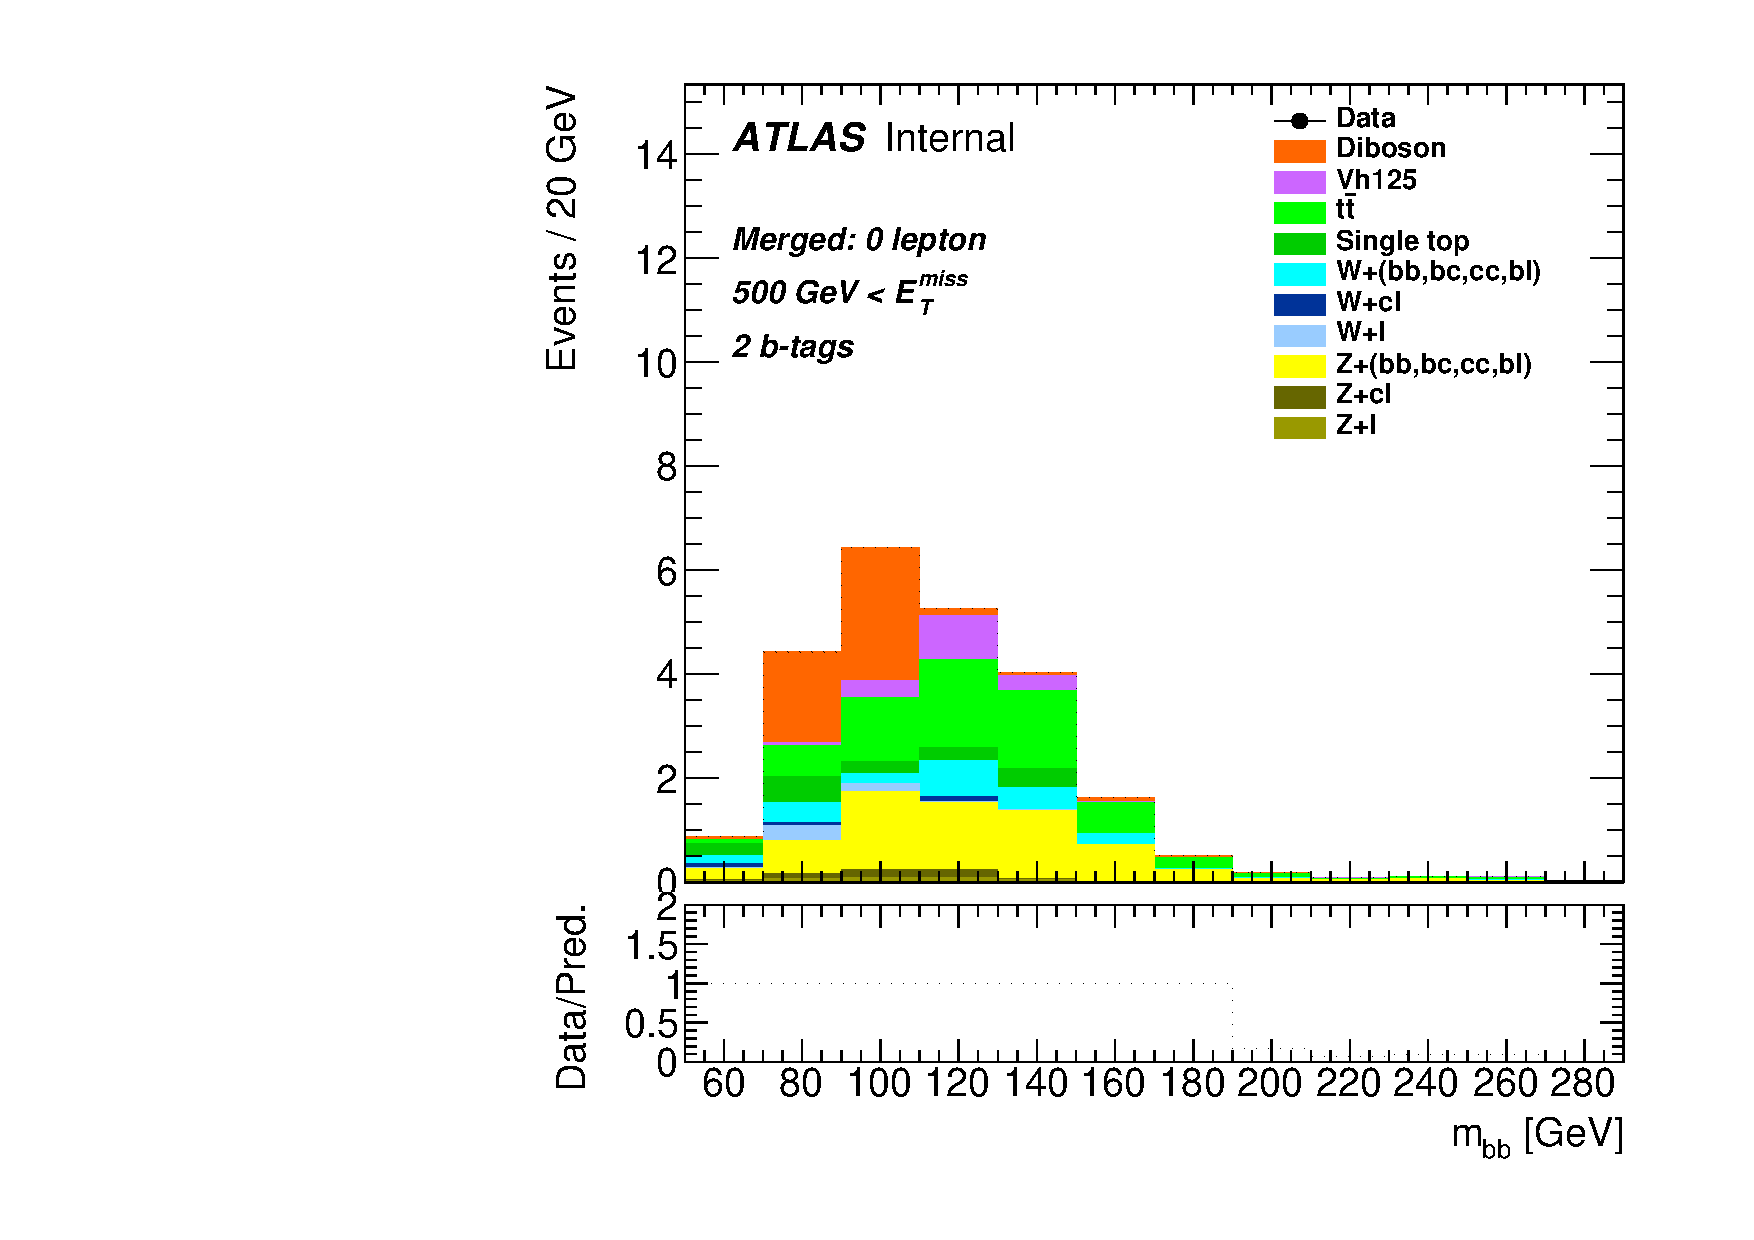
\includegraphics[width=0.4\textwidth]{appendices/figures/Region_BMin500_incFat1_Fat1_incJet1_Y2015_DSR_T2_L0_distmBB_J0_Prefit.pdf}
    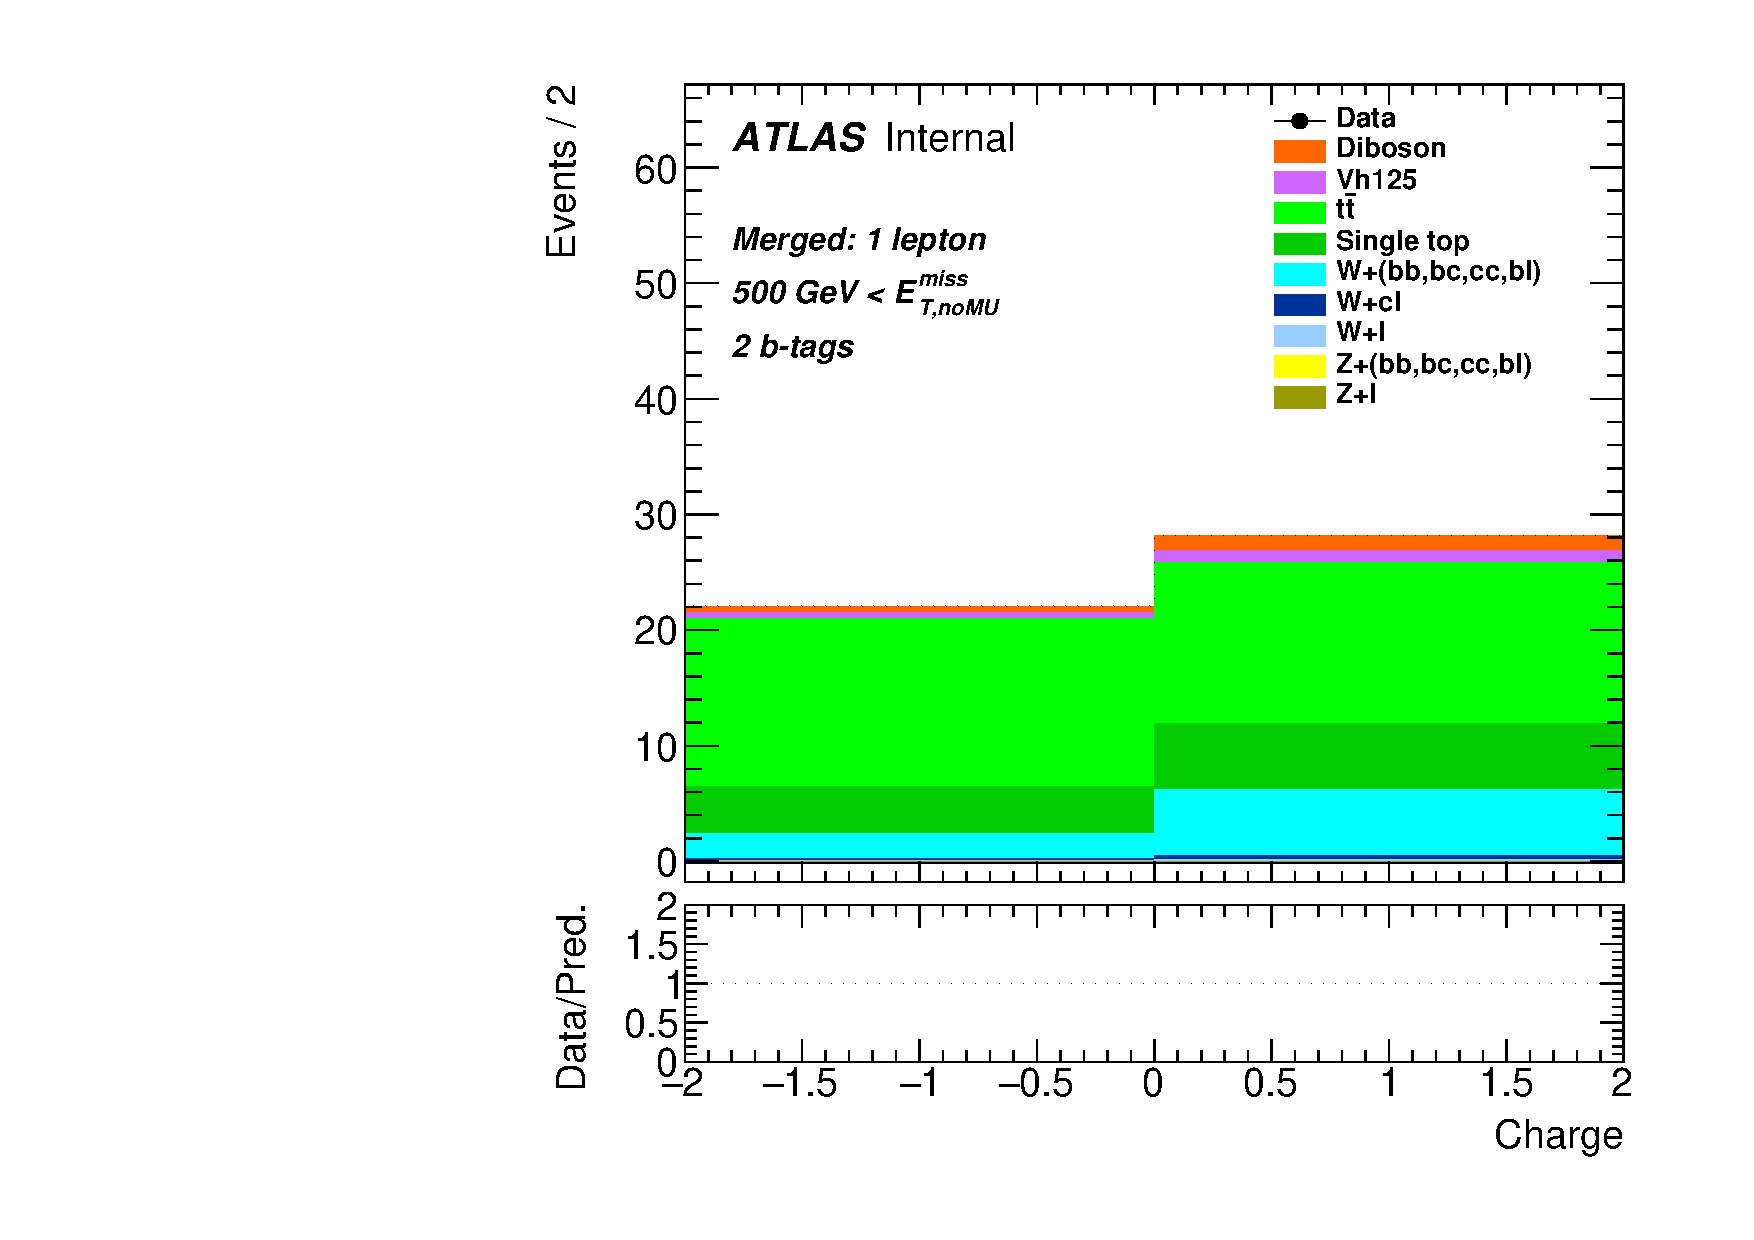
\includegraphics[width=0.4\textwidth]{appendices/figures/Region_BMin500_incFat1_Fat1_incJet1_Y2015_DCR1_T2_L1_distCharge_J0_Prefit.pdf}
    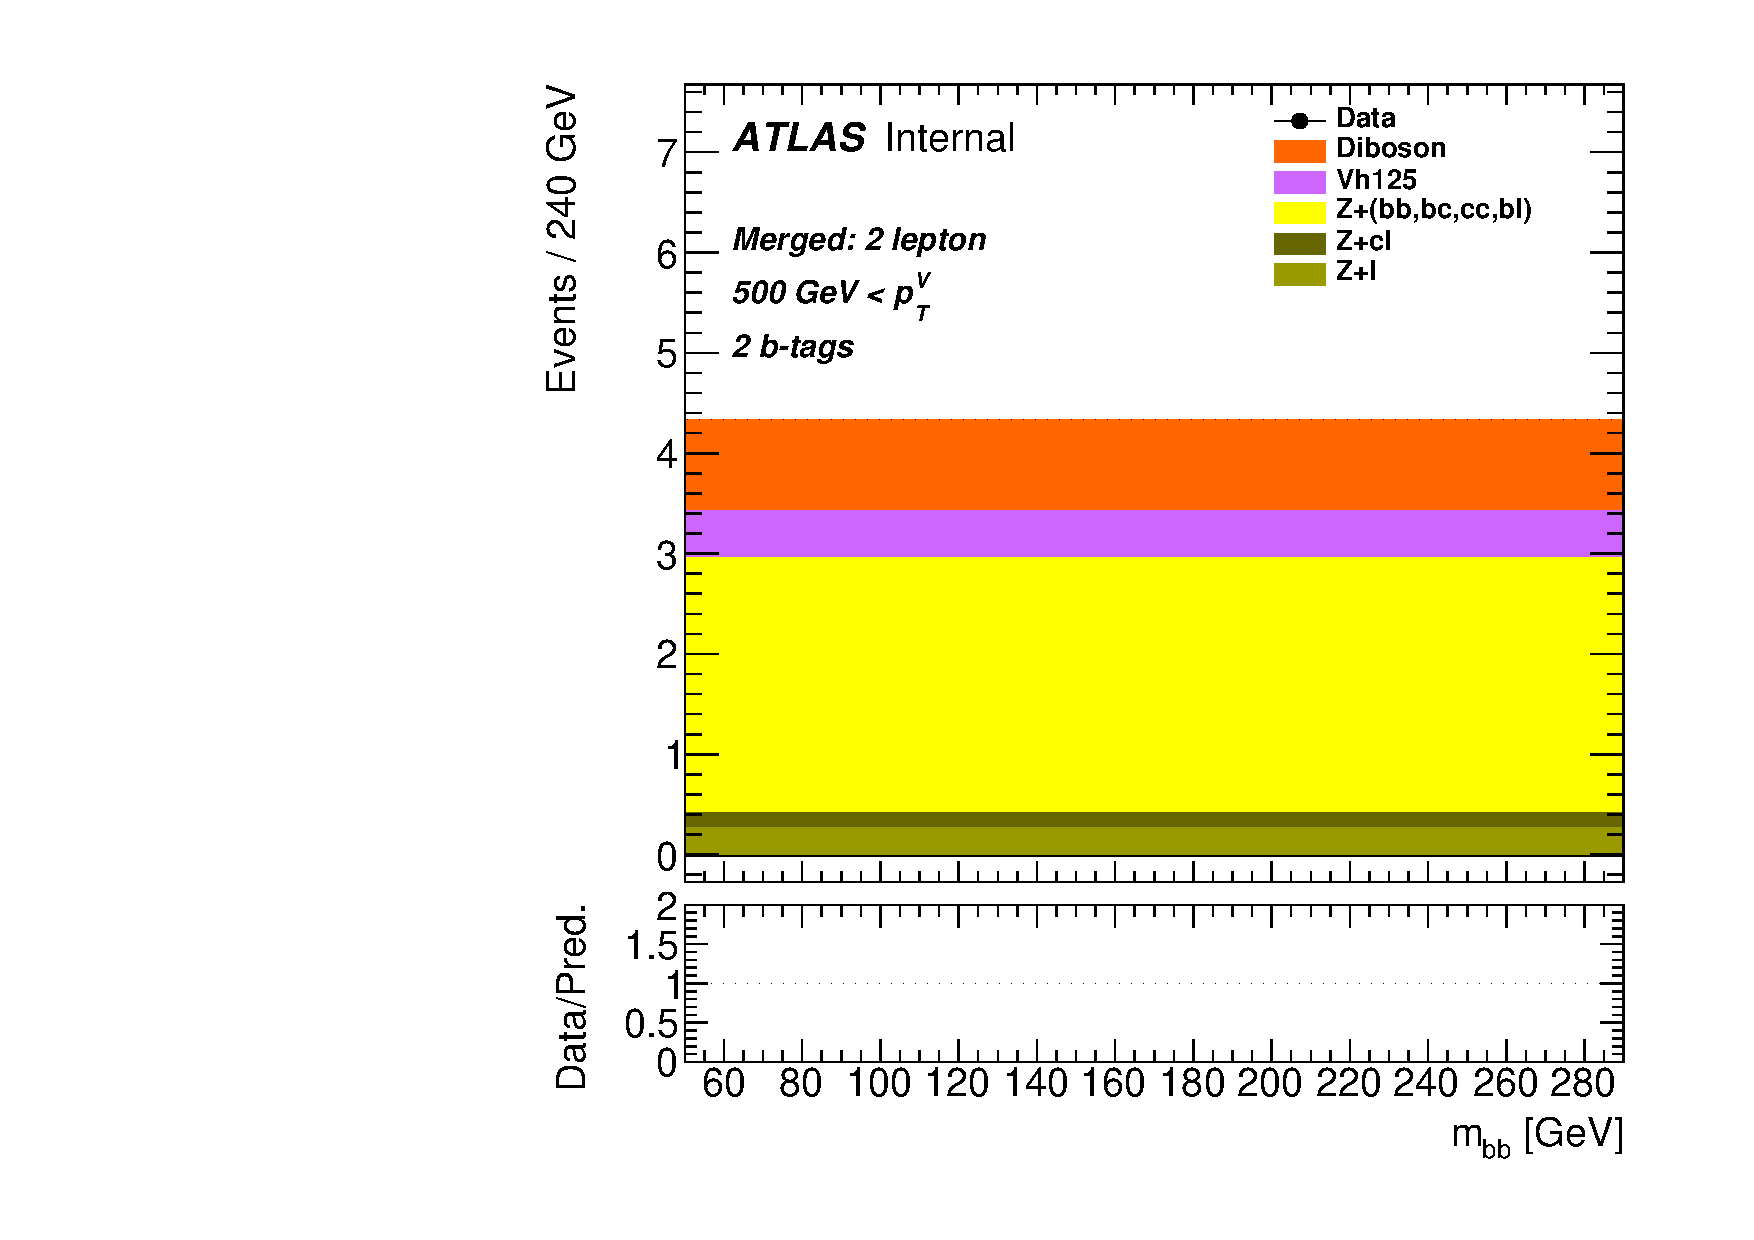
\includegraphics[width=0.4\textwidth]{appendices/figures/Region_BMin500_incFat1_Fat1_incJet1_Y2015_DCR2_T2_L2_distmBB_J0_Prefit.pdf}
    \caption{Large-R jet mass distribution in the 2-btagged singal and control regions.}
    \label{fig:fl_mj}
\end{figure}

\par Ideally, large-R jets selected by cutting on CombinedXbbScore are likely to have two b-hadorns ghost-associated to them and have a truch labeling of bb.

\par To have a clear look at the fraction of large-R jets labling, the Xbb tag fraction which refer to the fraction of large-R jets with labeling bb are examined for 1 lepton region with W+jets samples in Fig.\ref{fig:xbbw} and for 2 region with Z+jets samples in Fig.\ref{fig:xbbz}.

\begin{figure}[h]
    \centering
    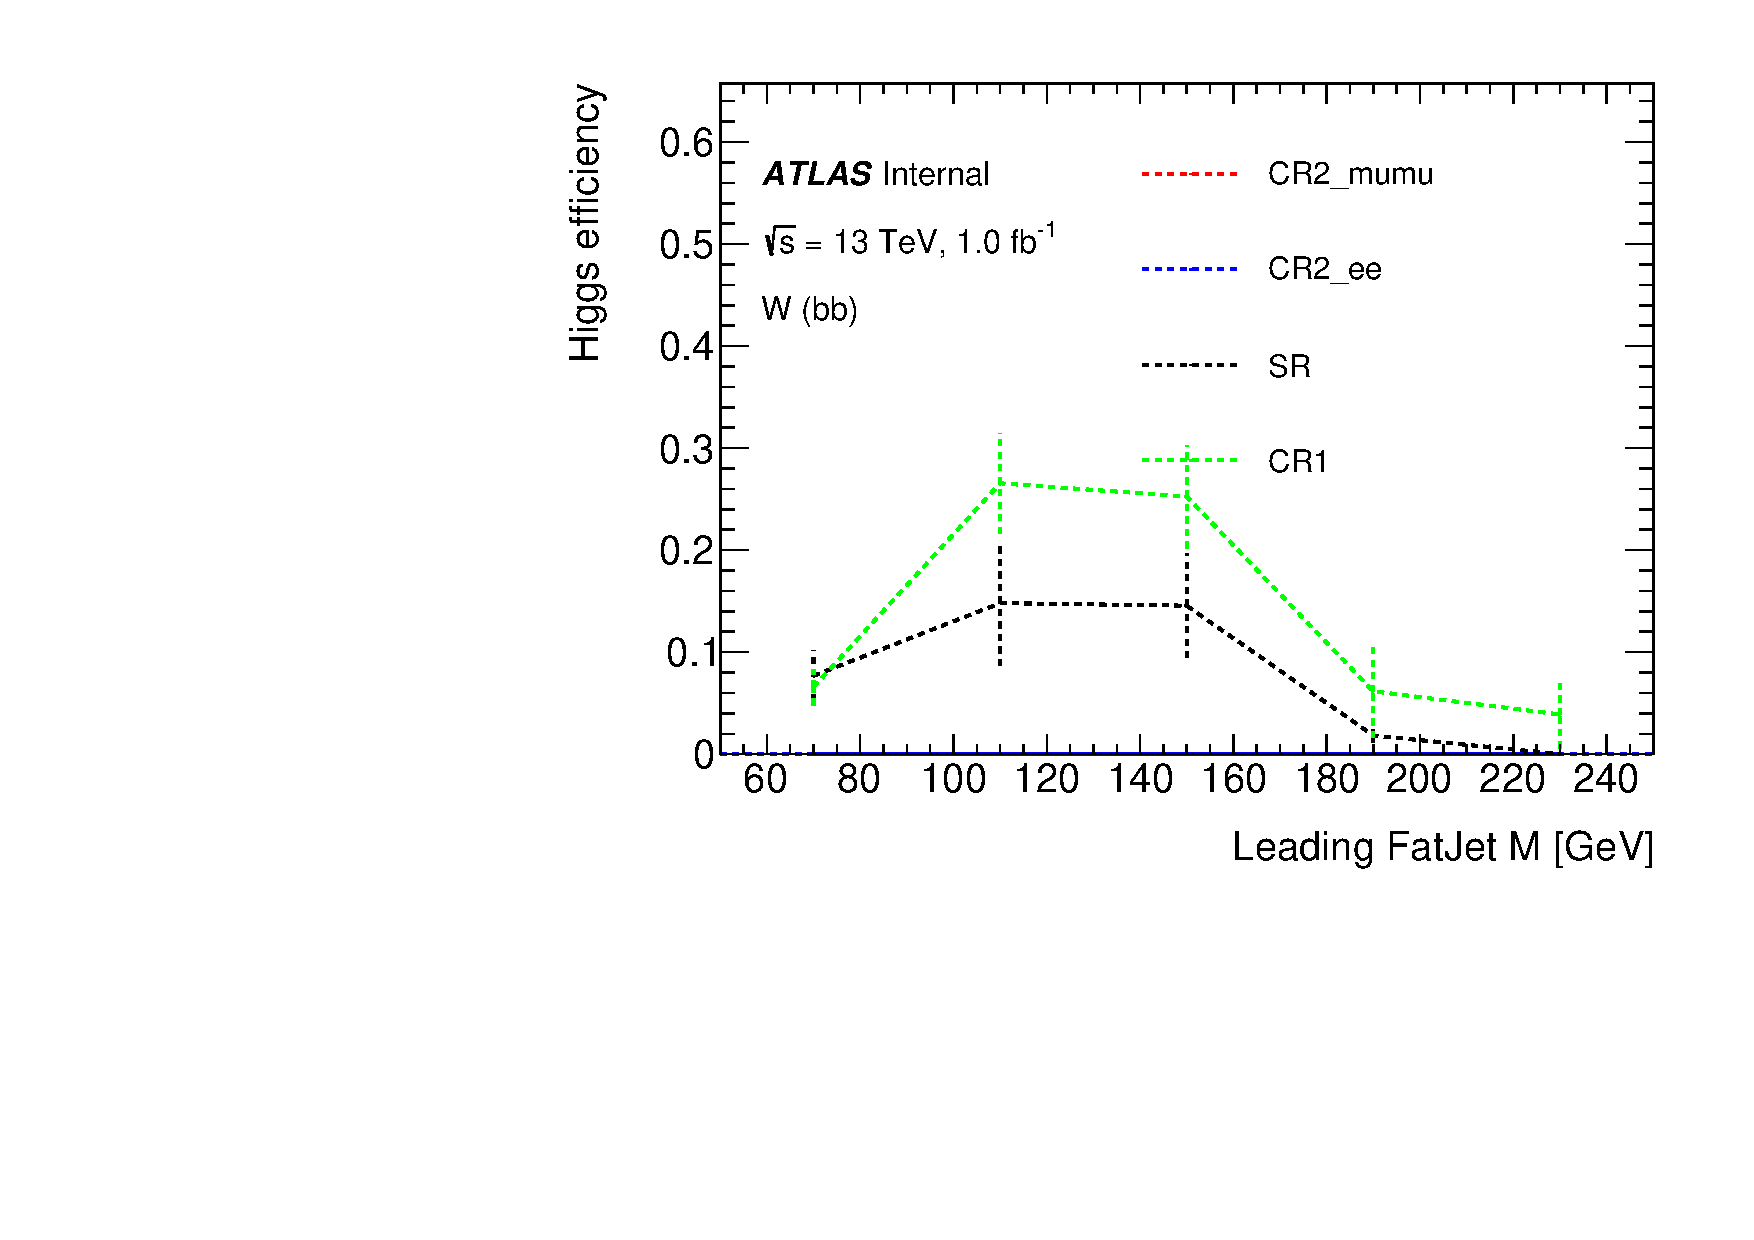
\includegraphics[width=0.45\textwidth]{appendices/figures/eff_W}
    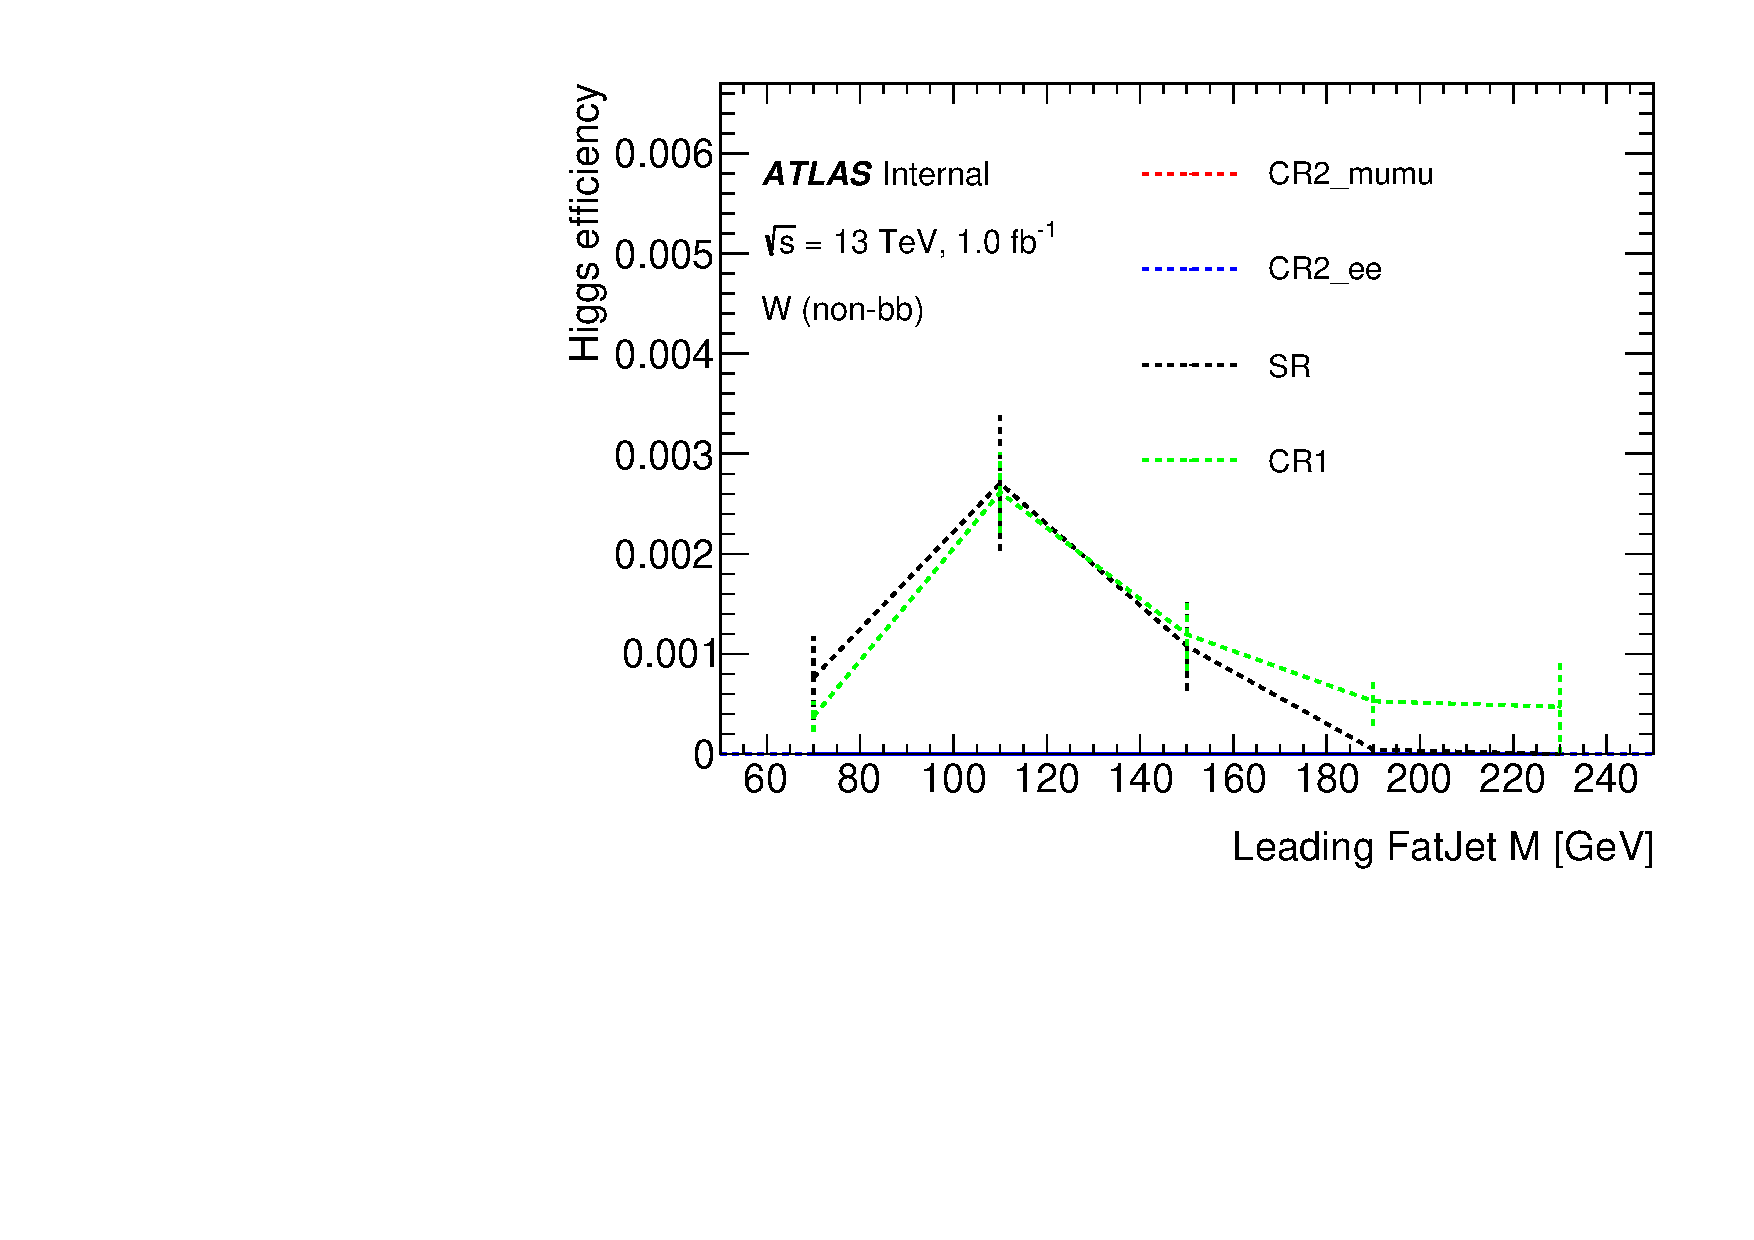
\includegraphics[width=0.45\textwidth]{appendices/figures/eff_Wnon}
    \caption{Fraction of large-R jets with bb labeling (left) and without bb labeling (right) in with W+jets samples.}
    \label{fig:xbbw}
\end{figure}

\begin{figure}[h]
    \centering
    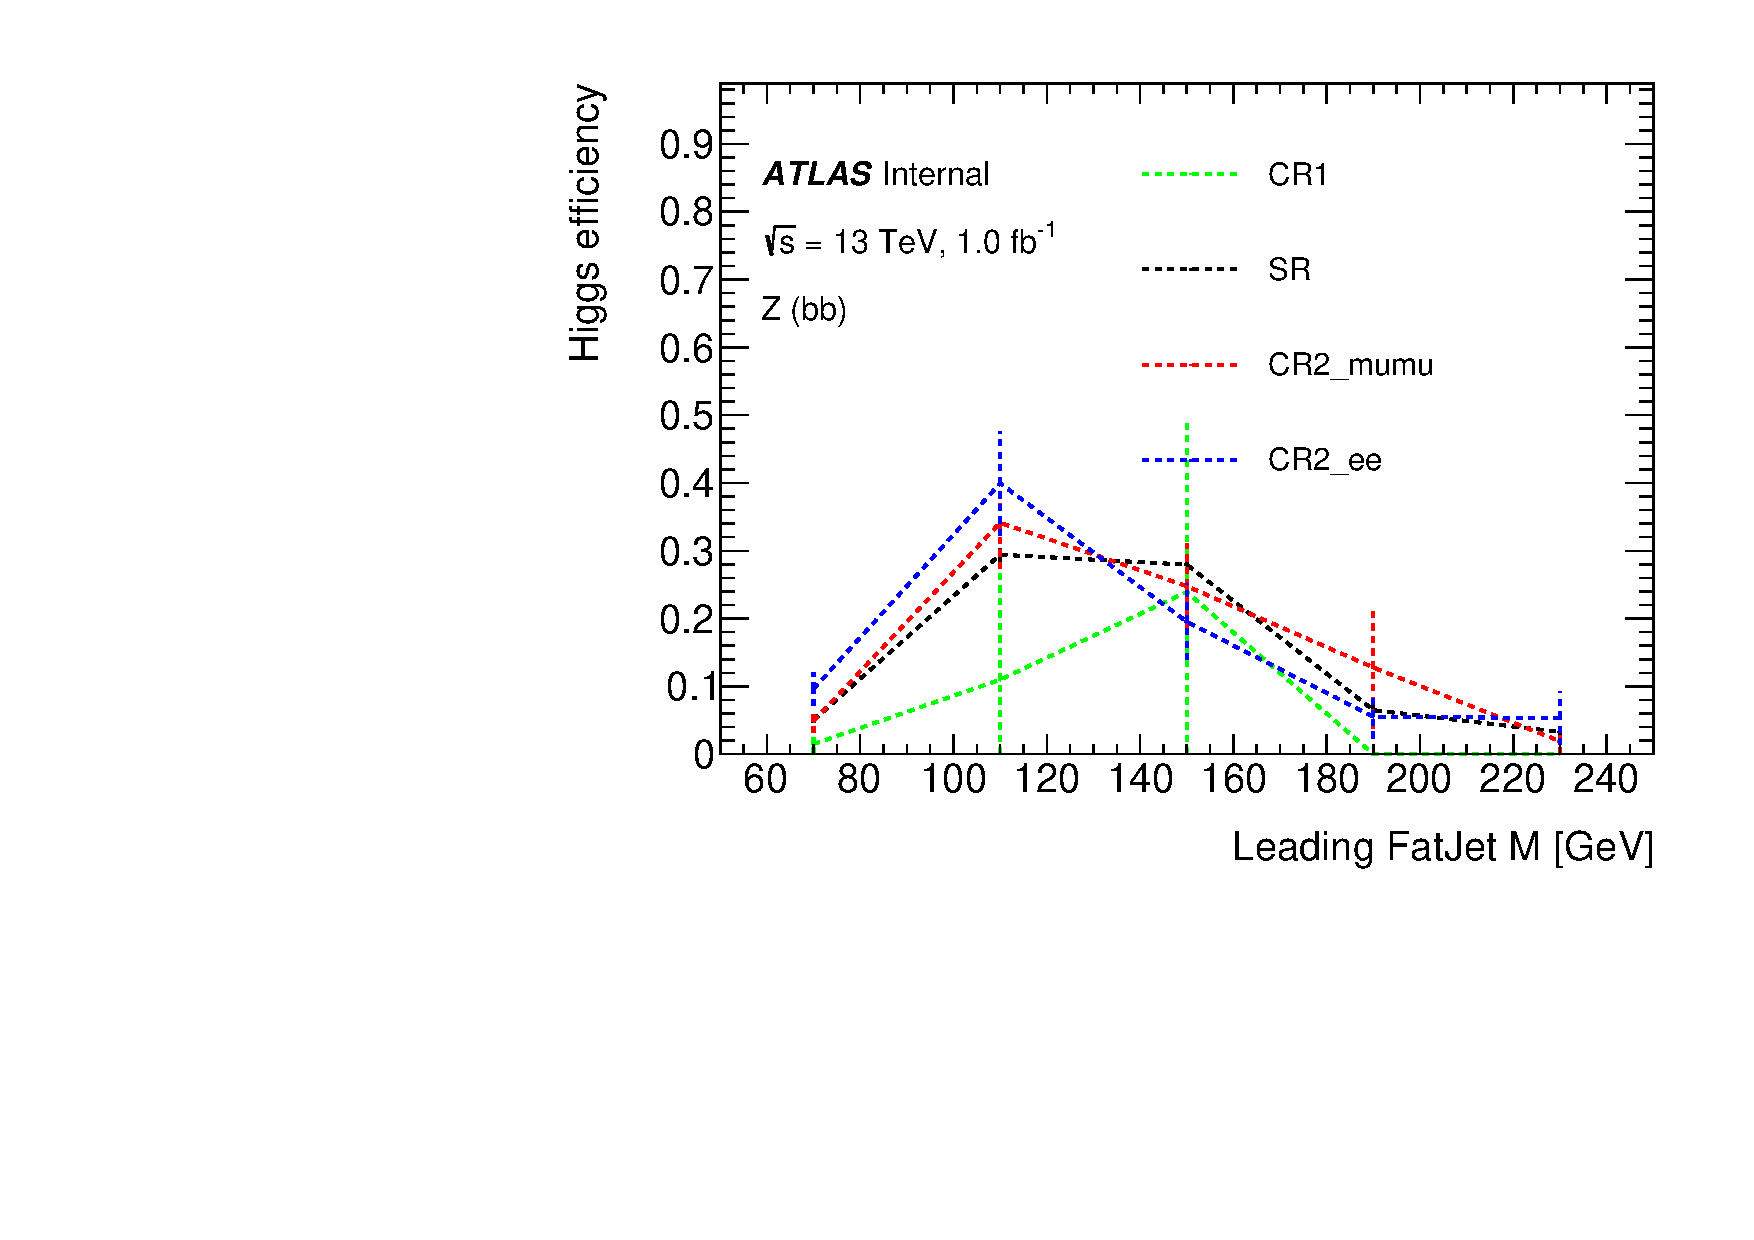
\includegraphics[width=0.45\textwidth]{appendices/figures/eff_Z}
    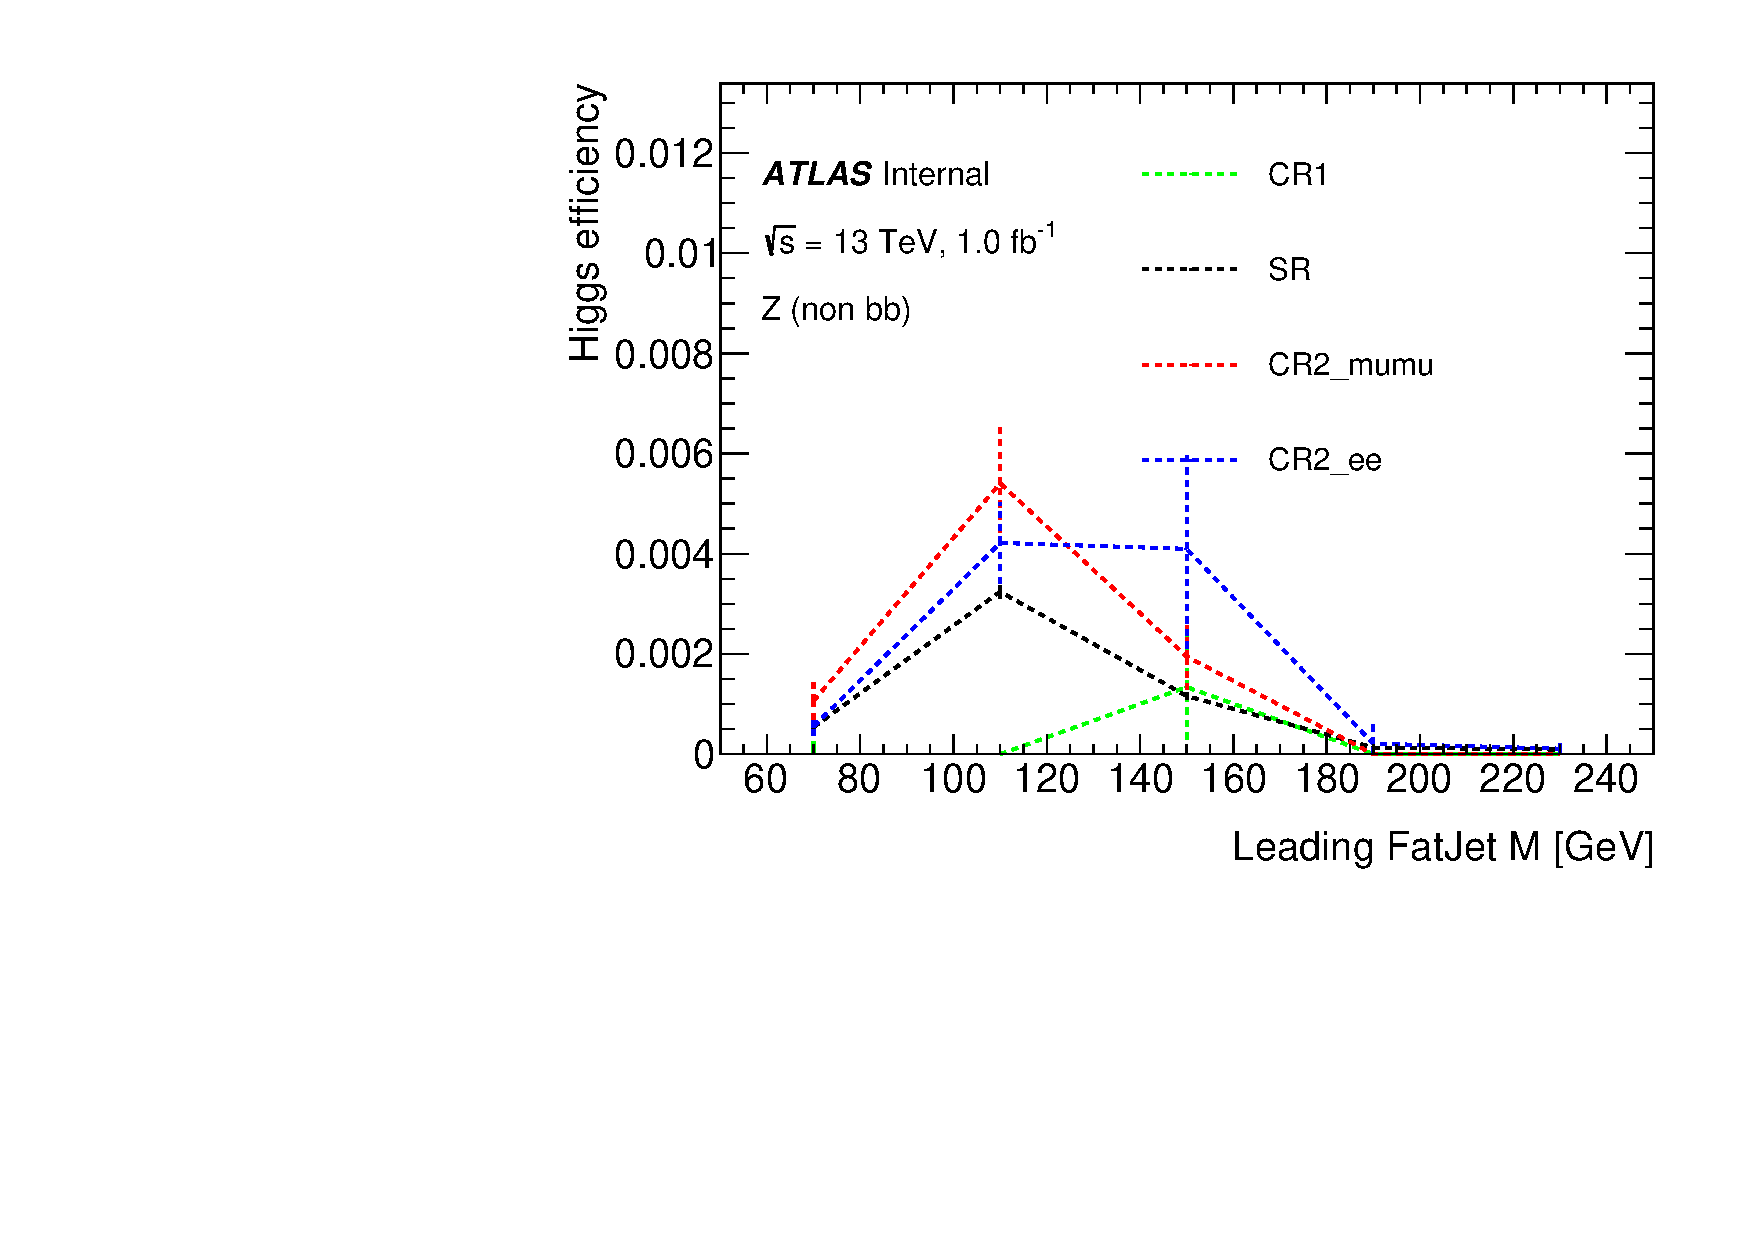
\includegraphics[width=0.45\textwidth]{appendices/figures/eff_Znon}
    \caption{Fraction of large-R jets with bb labeling (left) and without bb labeling (right) in with Z+jets samples.}
    \label{fig:xbbz}
\end{figure}

\par Xbb tag fraction of signal region vs 1b control regions in Fig.\ref{fig:xbbw} matches within uncertainty, as well as signal region vs 2b control regions in Fig.\ref{fig:xbbz}.
And the Xbb tag fraction peaks in around Higgs mass.

\par The flavor breakdown of backgrounds with truth labeling in singal and control regions is showed in Fig.\ref{fig:fl_pie}.

\begin{figure}[h]
    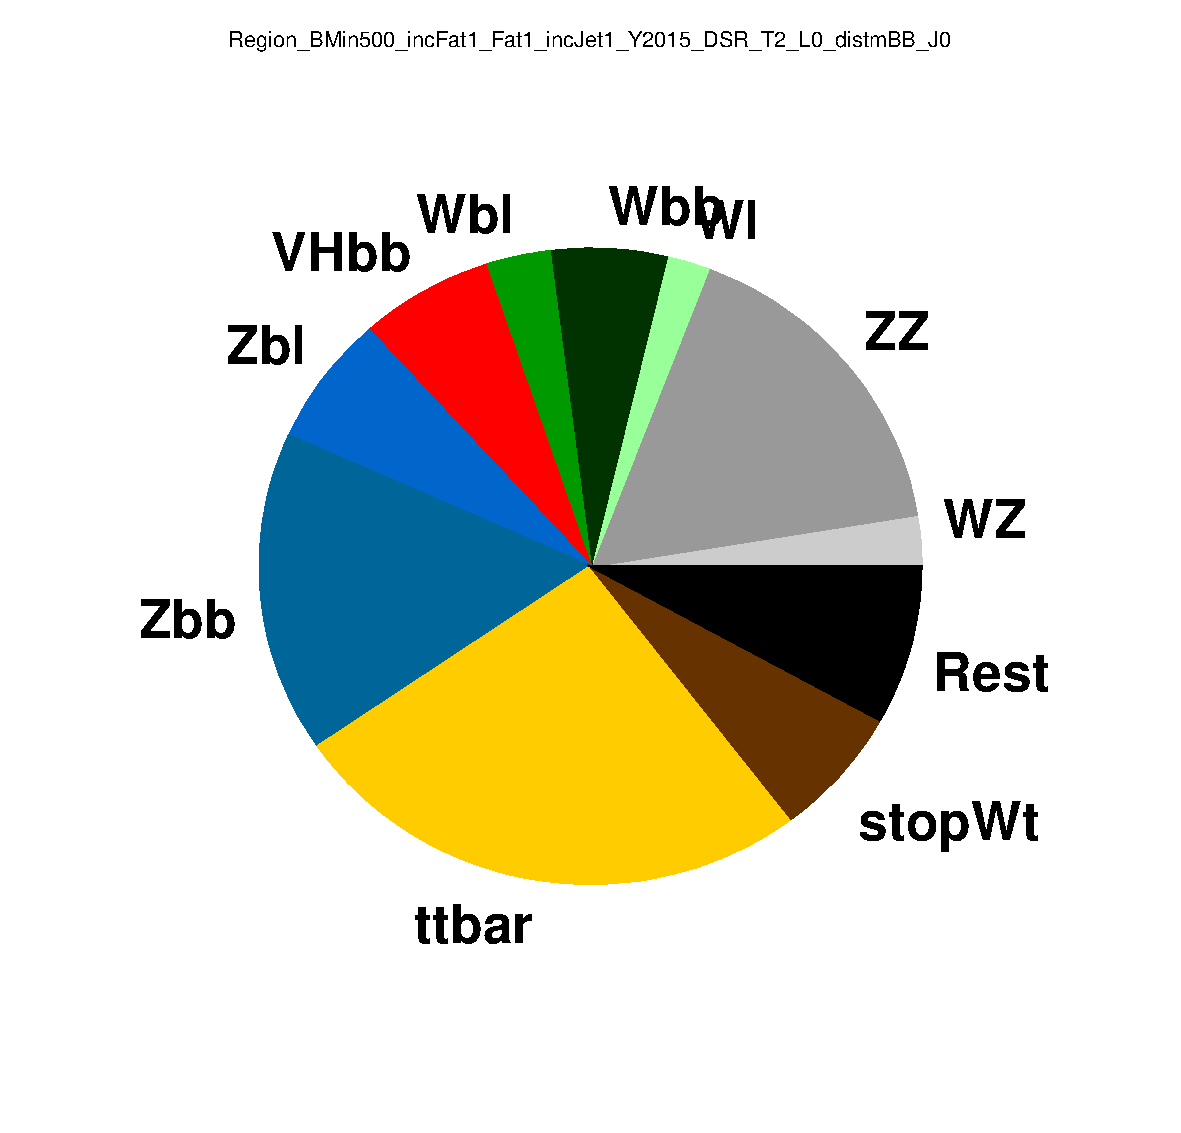
\includegraphics[ width=0.3\textwidth]{appendices/figures/pie0.pdf}
    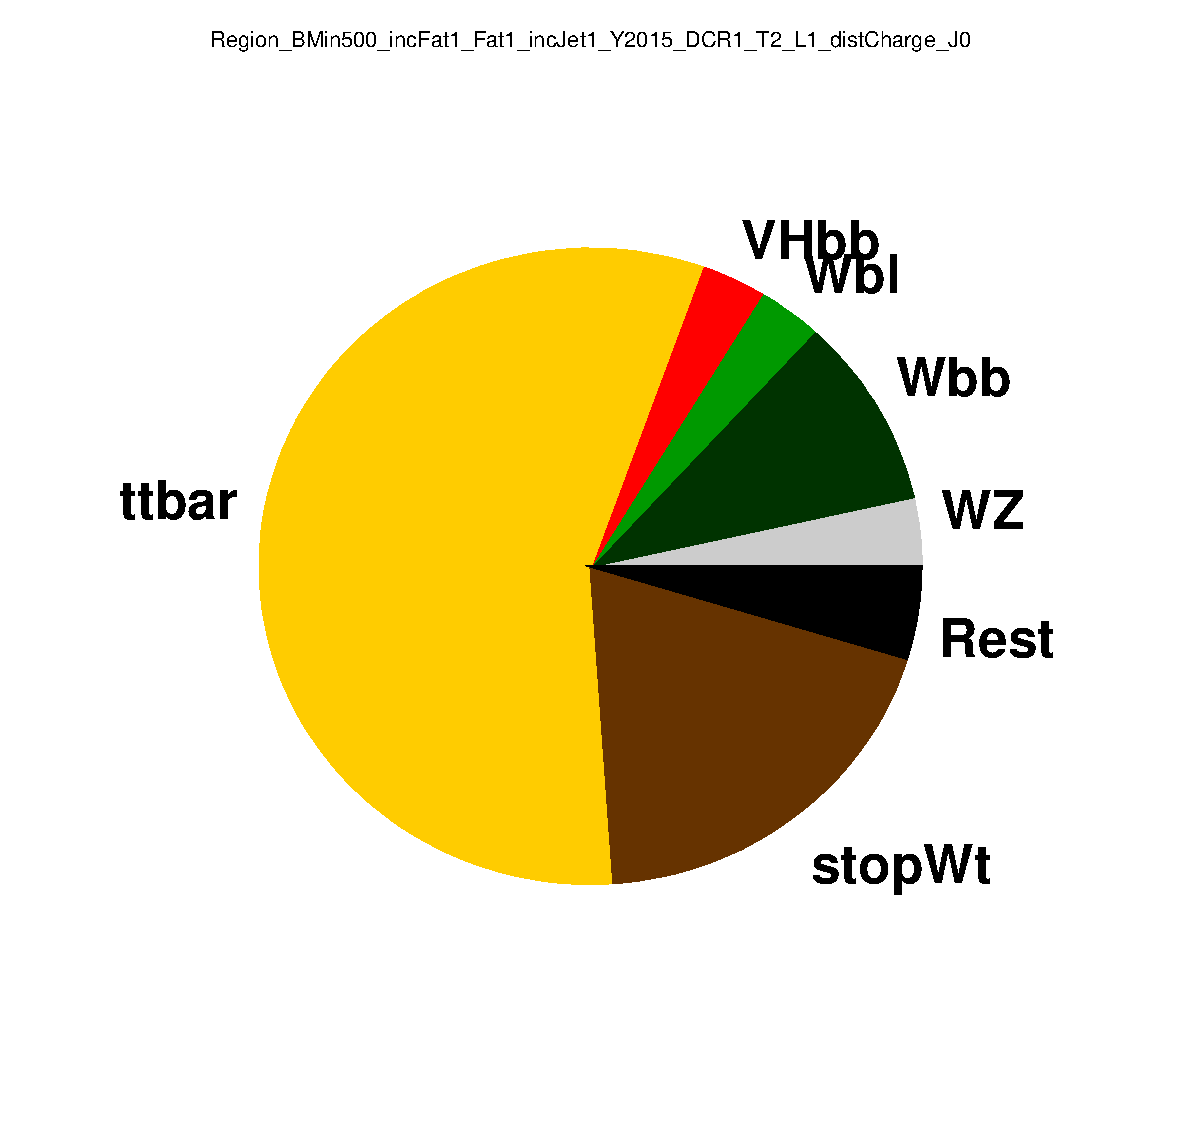
\includegraphics[ width=0.3\textwidth]{appendices/figures/pie1.pdf}
    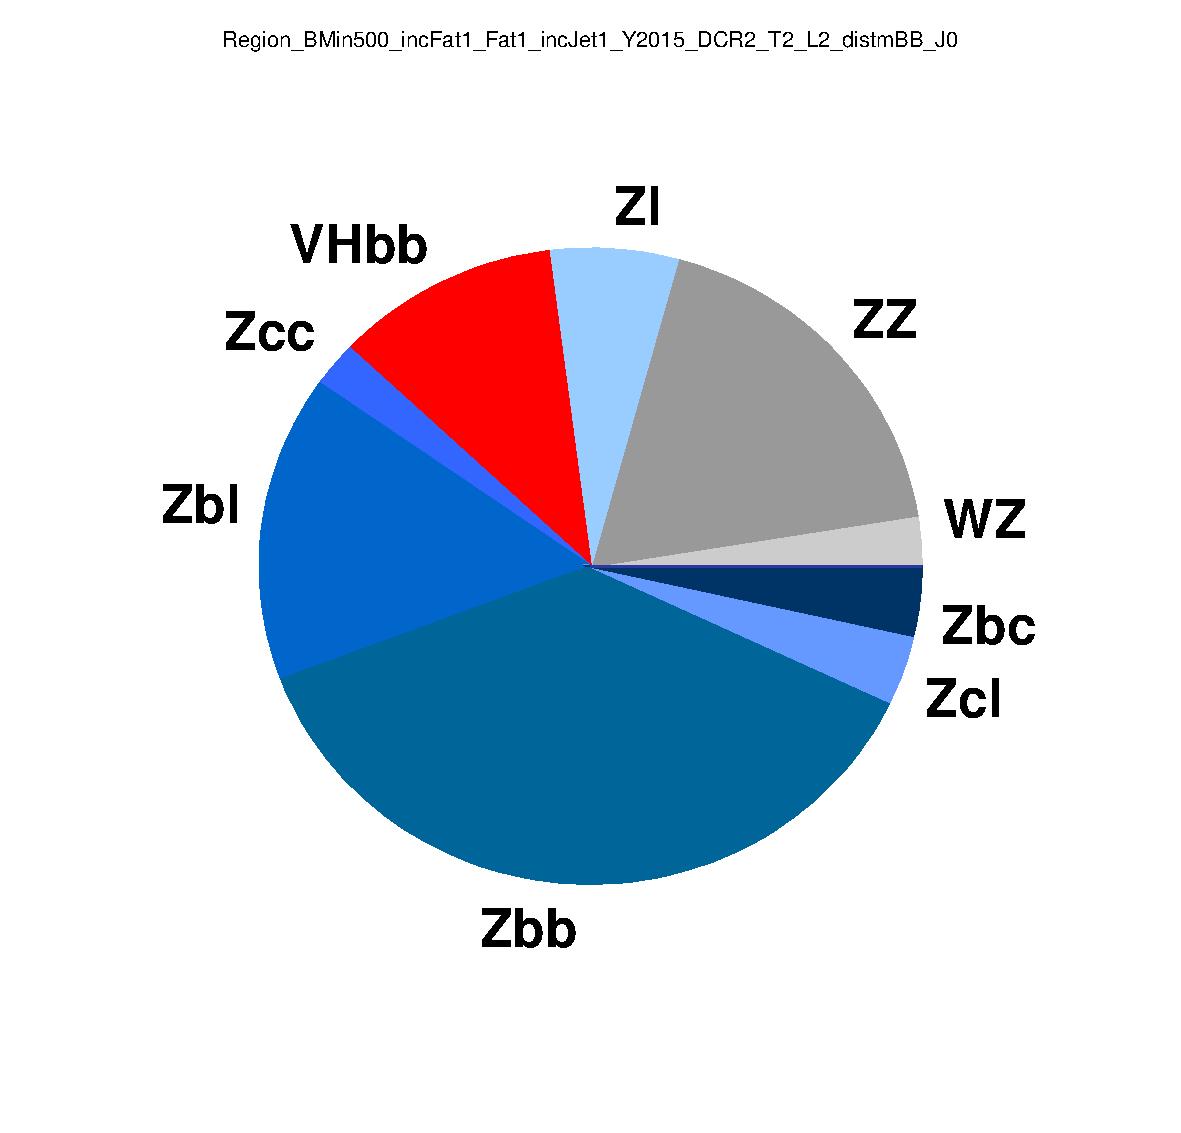
\includegraphics[ width=0.3\textwidth]{appendices/figures/pie2.pdf}
    \caption{Flavor breakdown of backgrounds with truth labeling in singal and control regions.}
    \label{fig:fl_pie}
\end{figure}

\par To further quantify the flavor breakdown in signal and control regions are showed in Table.\ref{tab:fl0}, Table.\ref{tab:fl1} and Table.\ref{tab:fl2}.

\begin{table}
    \centering
    \tiny
    \begin{tabular}{l|c|}
    \cline{2-2} & \multicolumn{1}{c|}{Zero lepton 2 tag merged,~$E_{T}^{miss}$$ >$ 500 GeV} \\
    \hline
    signal mzp1400\_mA600 & 0.0458$\pm$0.0005 \\
    \hline
    WZ    & 0.6106$\pm$0.2170 \\
    ZZ    & 3.9200$\pm$0.3486 \\
    Wl    & 0.4992$\pm$0.2104 \\
    Wcl   & 0.2709$\pm$0.0918 \\
    Wbb   & 1.3348$\pm$0.2478 \\
    Wbl   & 0.7481$\pm$0.1999 \\
    Wbc   & 0.0100$\pm$0.0070 \\
    Zl    & 0.3124$\pm$0.0293 \\
    VHbb  & 1.5404$\pm$0.0162 \\
    WW    & 0.1818$\pm$0.1285 \\
    Zcc   & 0.3775$\pm$0.0293 \\
    Zbl   & 1.5497$\pm$0.0580 \\
    Zbb   & 3.8587$\pm$0.0879 \\
    Zcl   & 0.4465$\pm$0.0431 \\
    Zbc   & 0.2807$\pm$0.0233 \\
    ttbar & 6.0874$\pm$0.2225 \\
    stopWt& 1.5491$\pm$0.4528 \\
    stops & 0.0200$\pm$0.0141 \\
    \hline
    Total Bkgd & 23.5977$\pm$3.3084 \\
    \hline
    \end{tabular}
    \caption{Flavor breakdown of backgrounds with truth labeling in singal region.}
    \label{tab:fl0}
\end{table}

\begin{table}
    \centering
    \tiny
    \begin{tabular}{l|c|}
        \cline{2-2} & \multicolumn{1}{c|}{One lepton 2 tag merged,~$E_{T}^{miss}$$ >$ 500 GeV} \\
        \hline
        WZ    & 1.7570$\pm$0.2641 \\
        ZZ    & 0.0775$\pm$0.0264 \\
        Wl    & 0.2212$\pm$0.0978 \\
        Wcl   & 0.5467$\pm$0.2127 \\
        Wbb   & 4.8836$\pm$0.5282 \\
        Wcc   & 0.5283$\pm$0.1443 \\
        Wbl   & 1.5783$\pm$0.2929 \\
        Wbc   & 0.8691$\pm$0.2415 \\
        Zl    & 0.0060$\pm$0.0043 \\
        VHbb  & 1.5967$\pm$0.0162 \\
        Zbl   & 0.0093$\pm$0.0093 \\
        Zbb   & 0.0333$\pm$0.0276 \\
        ttbar & 28.449$\pm$0.8372 \\
        stopWt& 9.6438$\pm$1.1237 \\
        stops & 0.0704$\pm$0.0321 \\
        \hline
        Total Bkgd & 50.2699$\pm$3.1672 \\
        \hline
    \end{tabular}
    \caption{Flavor breakdown of backgrounds with truth labeling in 1 lepton control region.}
    \label{tab:fl1}
\end{table}    

\begin{table}
    \centering
    \tiny
    \begin{tabular}{l|c|}
        \cline{2-2} & \multicolumn{1}{c|}{Two lepton 2 tag merged, $E_{T}^{miss}$ $>$ 500 GeV} \\
        \hline
        WZ    & 0.1108$\pm$0.0427 \\
        ZZ    & 0.7880$\pm$0.1048 \\
        Zl    & 0.2722$\pm$0.1364 \\
        VHbb  & 0.4736$\pm$0.0053 \\
        Zcc   & 0.0991$\pm$0.0360 \\
        Zbl   & 0.6740$\pm$0.0969 \\
        Zbb   & 1.6105$\pm$0.1363 \\
        Zcl   & 0.1514$\pm$0.0428 \\
        Zbc   & 0.1524$\pm$0.0404 \\
        \hline
        Total Bkgd & 4.3320$\pm$ 5.8464 \\
        \hline
    \end{tabular}
    \caption{Flavor breakdown of backgrounds with truth labeling in 2 lepton control region.}
    \label{tab:fl2}
\end{table}

\par According to the tables above, the Wbb fraction in W+jets in signal region is 46.62\% $\pm$ 10.76\% compared to 56.60\% $\pm$ 7.68\% in 1 lepton control reigon. 
And the Zbb fraction in Z+jets is 56.53\%$\pm$1.64\% compared to 54.42\%$\pm$6.21\% in 2 lepton control reigon.

\subsection{Preliminary significance study}

\par To quantify the improvement brought by the CombinedXbbScore, the signal significances of these two methods are compared.
Singal Significance in each bin is defined as
\begin{equation}
    S_i = \sqrt{2(s + b)ln(1 + \frac{s}{b}) − s},
\end{equation}
where s, b is the count of signal and background in the i-th bin.

\par And the Bin-by-bin signal significance is difined as
\begin{equation}
    S_{bin-by-bin} = \sqrt{\sum_i S_i^2}, 
\end{equation}

\par Fig.\ref{fig:ss_ratio} (left) shows the ratio of signal significance of the 2b region defined by CombinedXbbScore vs 2b b-tagged VR trackjets with the Higgs window [70, 140]~GeV,
while the right plot is without the Higgs window.
\begin{figure}[h]
    \centering
    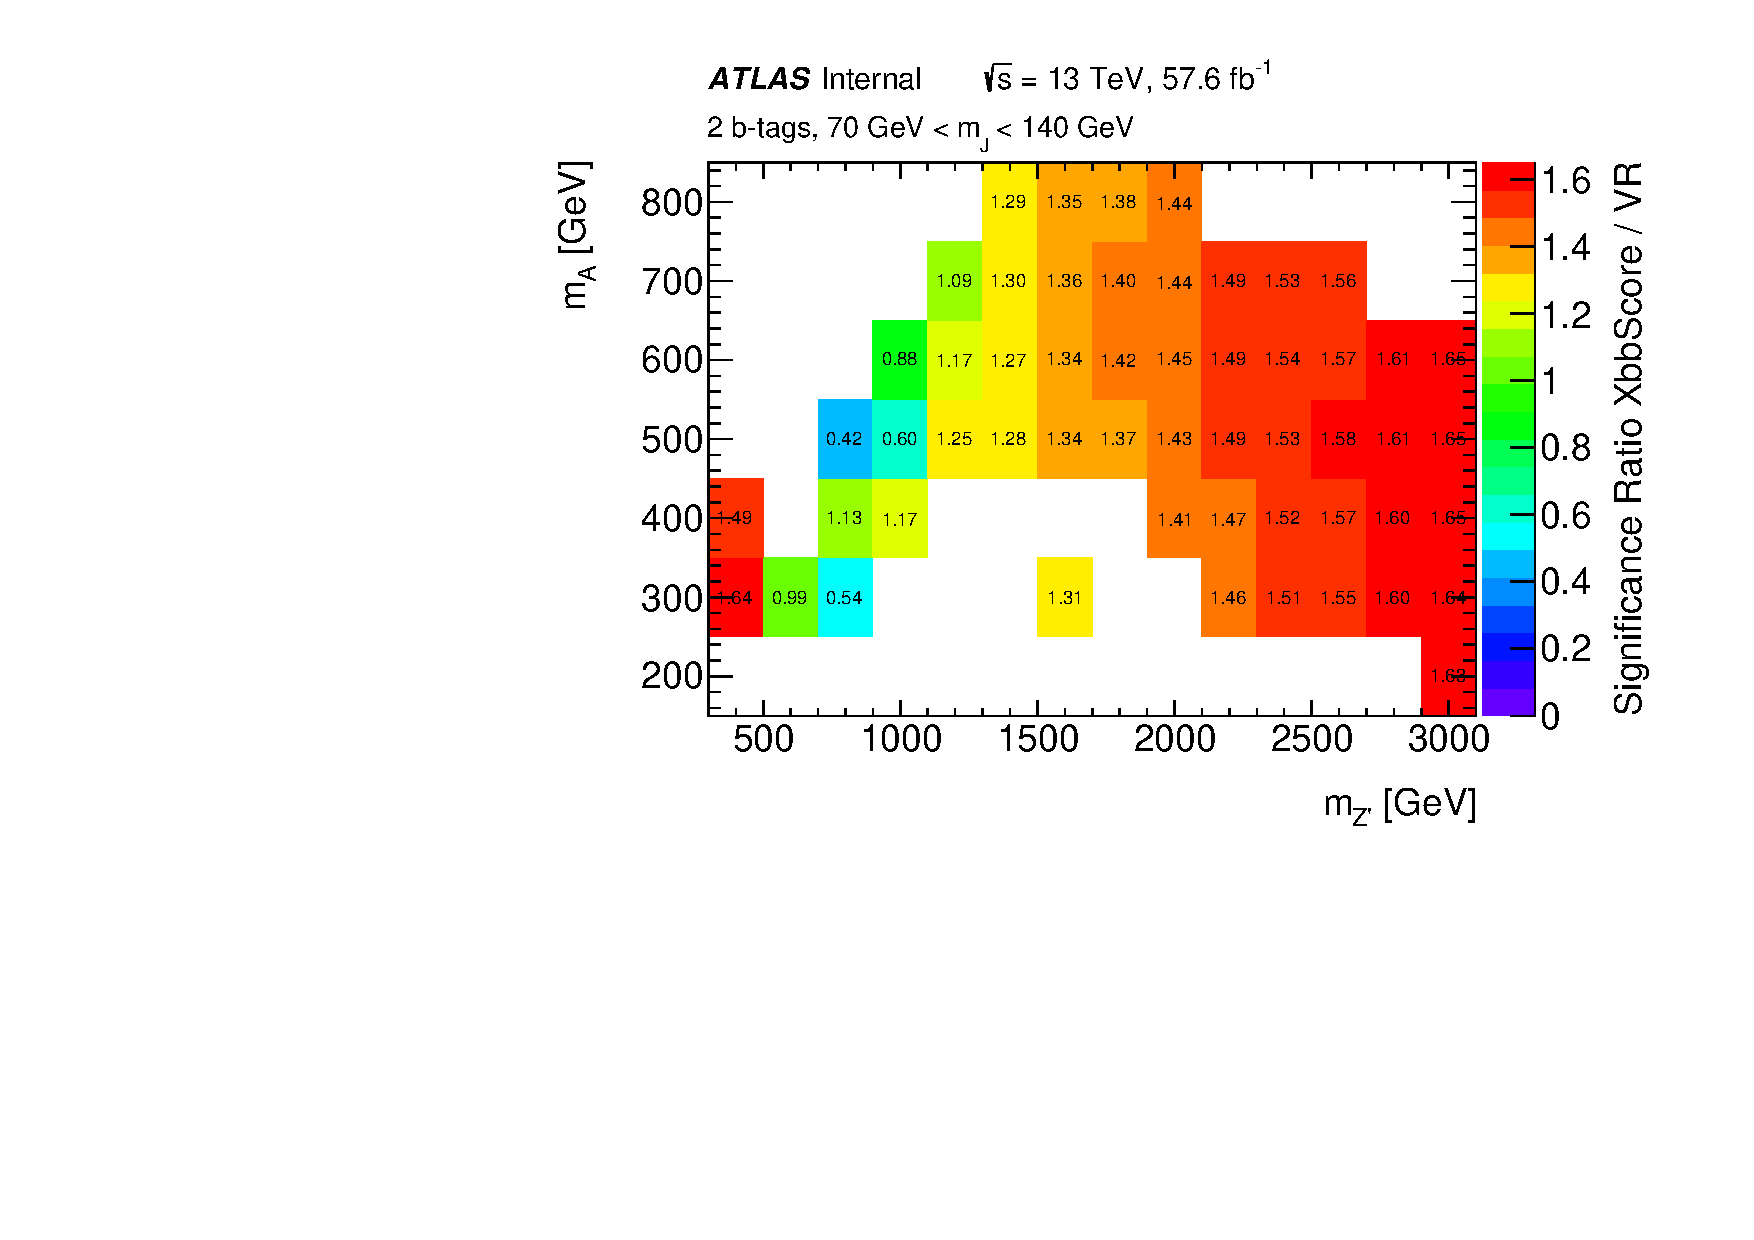
\includegraphics[width=0.45\textwidth]{appendices/figures/2b-tags_XbbScoreoverVR_HiggsWindow.pdf}
    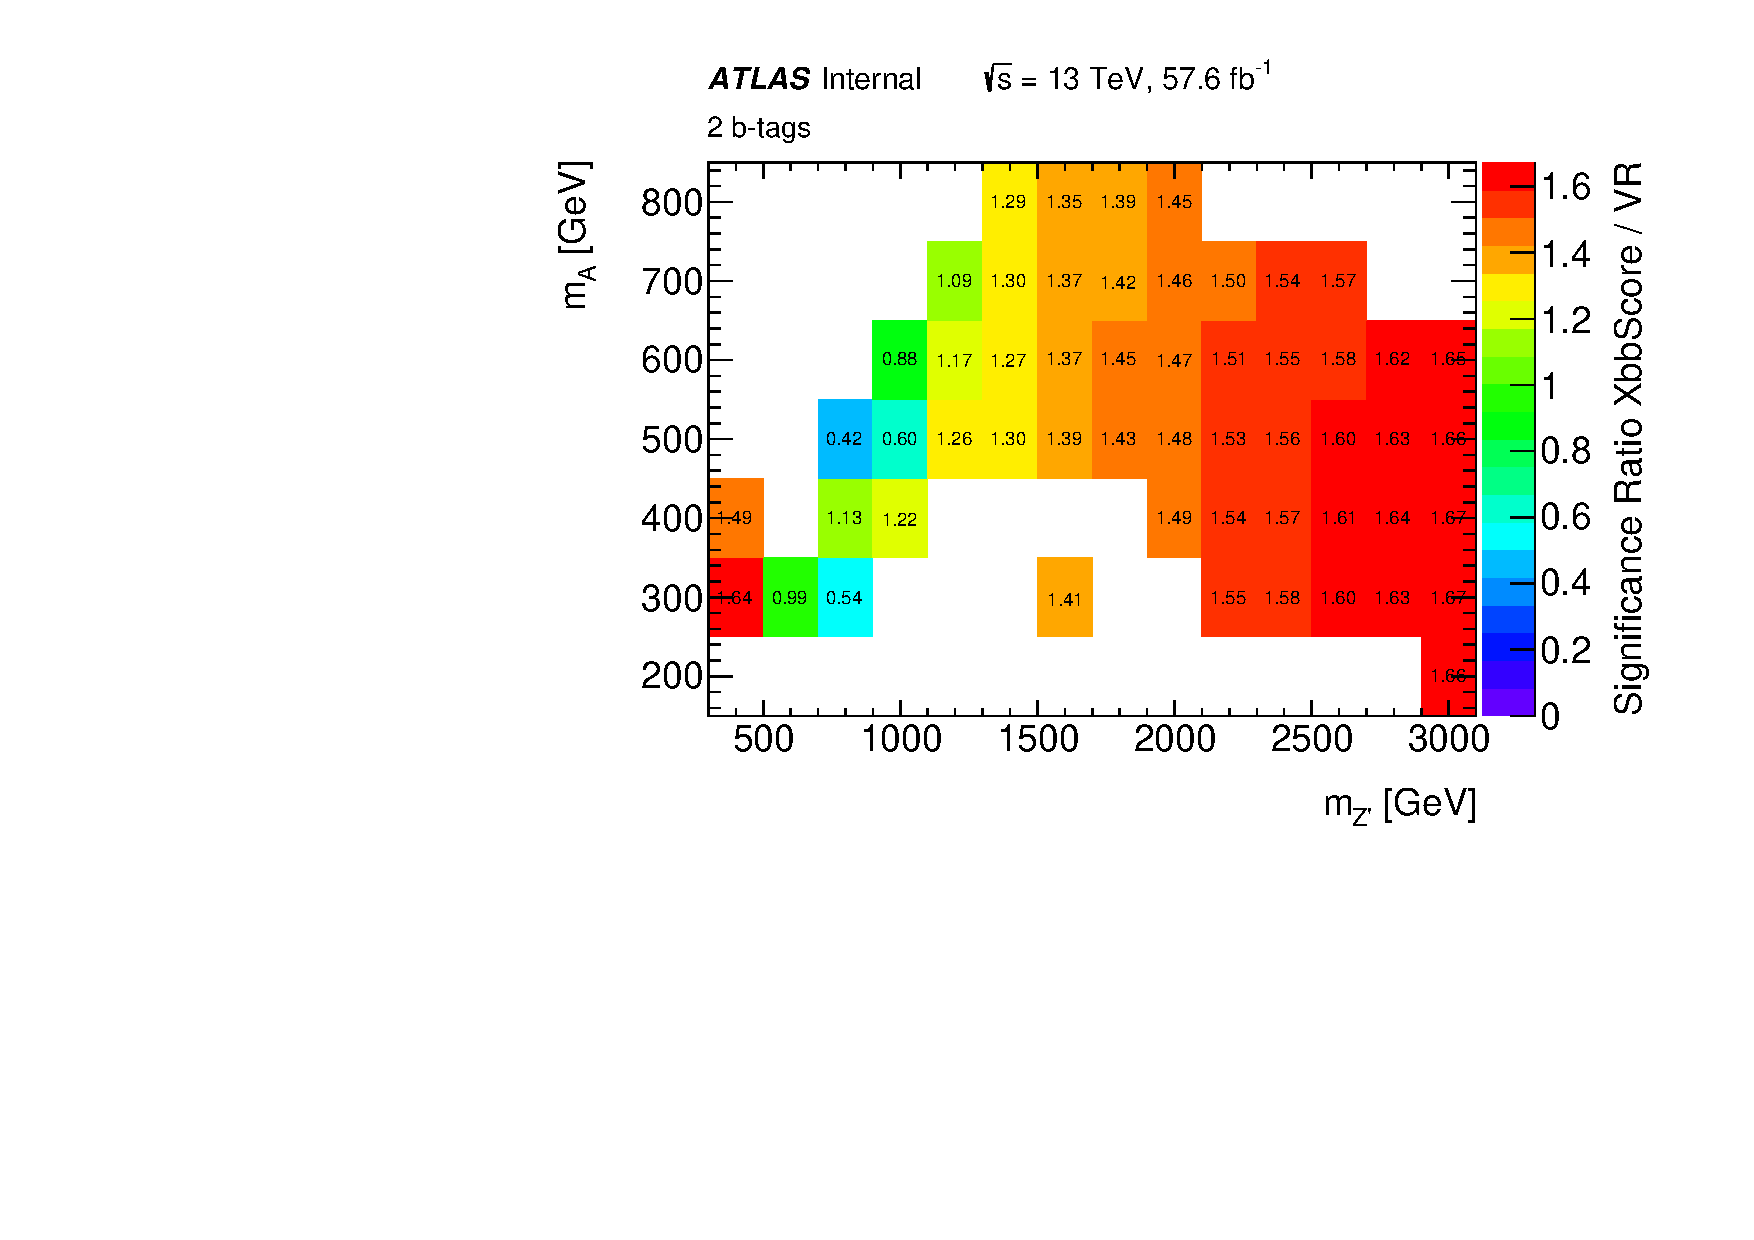
\includegraphics[width=0.45\textwidth]{appendices/figures/2b-tags_XbbScoreoverVR.pdf}
    \caption{Ratio of singal significance of 2b merged region defined by CombinedXbbScore compared to the orignal method with or without the Higgs window.}
    \label{fig:ss_ratio}
\end{figure}
